\documentclass[12pt, titlepage]{article}

\usepackage{booktabs}
\usepackage{tabularx}
\usepackage{hyperref}
\hypersetup{
    colorlinks,
    citecolor=black,
    filecolor=black,
    linkcolor=red,
    urlcolor=blue
}
\usepackage[round]{natbib}
\usepackage{mdframed}
\usepackage{enumitem}
\usepackage{parskip}
\usepackage{array}        
\usepackage{booktabs}  
\usepackage{graphicx}
\usepackage{svg}
\usepackage{longtable}  
\usepackage{float}      
\usepackage{geometry}   
\usepackage{pdflscape}  

%% Comments

\usepackage{color}

\newif\ifcomments\commentstrue %displays comments
%\newif\ifcomments\commentsfalse %so that comments do not display

\ifcomments
\newcommand{\authornote}[3]{\textcolor{#1}{[#3 ---#2]}}
\newcommand{\todo}[1]{\textcolor{red}{[TODO: #1]}}
\else
\newcommand{\authornote}[3]{}
\newcommand{\todo}[1]{}
\fi

\newcommand{\wss}[1]{\authornote{blue}{SS}{#1}} 
\newcommand{\plt}[1]{\authornote{magenta}{TPLT}{#1}} %For explanation of the template
\newcommand{\an}[1]{\authornote{cyan}{Author}{#1}}

%% Common Parts

\newcommand{\progname}{Software Engineering} % PUT YOUR PROGRAM NAME HERE
\newcommand{\authname}{Team \#22, TeleHealth Insights
\\ Mitchell Weingust
\\ Parisha Nizam
\\ Promish Kandel
\\ Jasmine Sun-Hu} % AUTHOR NAMES                  

\usepackage{hyperref}
    \hypersetup{colorlinks=true, linkcolor=blue, citecolor=blue, filecolor=blue,
                urlcolor=blue, unicode=false}
    \urlstyle{same}
                                


\begin{document}

\title{Verification and Validation Report: \progname} 
\author{\authname}
\date{\today}
	
\maketitle

\pagenumbering{roman}

\section{Revision History}

\begin{table}[hp]
  \caption{Revision History} \label{TblRevisionHistory}
  \begin{tabularx}{\textwidth}{p{1.5cm}p{1cm}p{3.5cm}X}
  \toprule {\textbf{Date}} & {\textbf{Vers.}} & {\textbf{Contributors}} & {\textbf{Notes}}\\
  \midrule
  3/10/25 & 1.0 & Mitchell Weingust & Added:\begin{itemize}[leftmargin=*]
    \item 4.2 Usability and Humanity
    \item 4.4 Operational and Environmental
    \item 7 - Changes Due to Testing
    \item 11 - Code Coverage Metrics
  \end{itemize}\\
  \bottomrule
  \end{tabularx}
  \end{table}

~\newpage

\section{Symbols, Abbreviations and Acronyms}

\renewcommand{\arraystretch}{1.2}
\begin{tabular}{l l} 
  \toprule		
  \textbf{symbol} & \textbf{description}\\
  \midrule 
  T & Test\\
  \bottomrule
\end{tabular}\\

\wss{symbols, abbreviations or acronyms -- you can reference the SRS tables if needed}

\newpage

\tableofcontents

\listoftables %if appropriate

\listoffigures %if appropriate

\newpage

\pagenumbering{arabic}

\hspace{2em}This document contains the team's verification and validation report for the TeleHealth
Insights project. This document features functional requirements evaluation, nonfunctional requirements
evaluation, unit testing, changes due to testing, automated testing, trace to requirements, trace to modules,
and code coverage metrics.

\section{Functional Requirements Evaluation}
\hspace{2em}The following section covers all the functional requirements tests specified in the project's
VnV Plan document. The coverage can be traced in Table X.

\subsection{Authentication}
\hspace{2em}The test results below focus on ensuring users can safely and securely login, create and
access their accounts without worrying about others accessing their information.

\begin{mdframed}[linewidth=0.5mm] \par
  \textbf{Test Case Identifier:} FR-ST-A1 \par
  \textbf{Input:} Selection of Parent account role for login \par
  \textbf{Expected Output:} The expected result is the Parent account role is selected and User is brought to the Parent login screen \par
  \textbf{Actual Output:} The actual result is the Parent account role is selected and User is brought to the Parent login screen \par
  \textbf{Expected and Actual Output Match:} True \par
  \textbf{Relevant Functional Requirement(s):} FR-A1
\end{mdframed}

\begin{mdframed}[linewidth=0.5mm] \par
  \textbf{Test Case Identifier:} FR-ST-A2 \par
  \textbf{Input:} Selection of Clinician account role for login \par
  \textbf{Expected Output:} The expected result is the Clinician account role is selected and User is brought to the Clinician login screen \par
  \textbf{Actual Output:} The actual result is the Clinician account role is selected and User is brought to the Clinician login screen \par
  \textbf{Expected and Actual Output Match:} True \par
  \textbf{Relevant Functional Requirement(s):} FR-A1
\end{mdframed}

\begin{mdframed}[linewidth=0.5mm] \par
  \textbf{Test Case Identifier:} FR-ST-A3 \par
  \textbf{Input:} Selection of 'Create Account', with a username that does not exist in the database, upon attempting to access the system \par
  \textbf{Expected Output:} The expected result is a new Parent account is created \par
  \textbf{Actual Output:} The actual result is a new Parent account is created \par
  \textbf{Expected and Actual Output Match:} True \par
  \textbf{Relevant Functional Requirement(s):} FR-A2
\end{mdframed}

\begin{mdframed}[linewidth=0.5mm] \par
  \textbf{Test Case Identifier:} FR-ST-A4 \par
  \textbf{Input:} Selection of 'Create Account', with a username that exists in the database, upon attempting to access the system \par
  \textbf{Expected Output:} The expected result is a new Parent account fails to be created \par
  \textbf{Actual Output:} The actual result is a new Parent account fails to be created \par
  \textbf{Expected and Actual Output Match:} True \par
  \textbf{Relevant Functional Requirement(s):} FR-A2
\end{mdframed}

\begin{mdframed}[linewidth=0.5mm] \par
  \textbf{Test Case Identifier:} FR-ST-A5 \par
  \textbf{Input:} Admin user selects option to ’Create Account’, with a username that does
  not exist in the database, upon attempting to access the system \par
  \textbf{Expected Output:} The expected result is a new Clinician account is created \par
  \textbf{Actual Output:} The actual result is a new Clinician account is created \par
  \textbf{Expected and Actual Output Match:} True \par
  \textbf{Relevant Functional Requirement(s):} FR-A3
\end{mdframed}

\begin{mdframed}[linewidth=0.5mm] \par
  \textbf{Test Case Identifier:} FR-ST-A6 \par
  \textbf{Input:} Admin user selects option to ’Create Account’, with a username that exists
  in the database, upon attempting to access the system \par
  \textbf{Expected Output:} The expected result is a new Clinician account fails to be created \par
  \textbf{Actual Output:} The actual result is a new Clinician account fails to be created \par
  \textbf{Expected and Actual Output Match:} True \par
  \textbf{Relevant Functional Requirement(s):} FR-A3
\end{mdframed}

\begin{mdframed}[linewidth=0.5mm] \par
  \textbf{Test Case Identifier:} FR-ST-A7 \par
  \textbf{Input:} Unique username and corresponding password that exists in the database \par
  \textbf{Expected Output:} The expected result is a successful login to a user’s account \par
  \textbf{Actual Output:} The actual result is a successful login to a user’s account \par
  \textbf{Expected and Actual Output Match:} True \par
  \textbf{Relevant Functional Requirement(s):} FR-A4
\end{mdframed}

\begin{mdframed}[linewidth=0.5mm] \par
  \textbf{Test Case Identifier:} FR-ST-A8 \par
  \textbf{Input:}Selection of 'logout' \par
  \textbf{Expected Output:} The expected result is a successful logout from a user’s account \par
  \textbf{Actual Output:} The actual result is a successful logout from a user’s account\par
  \textbf{Expected and Actual Output Match:} True \par
  \textbf{Relevant Functional Requirement(s):} FR-A5
\end{mdframed}

\subsection{Data Collection and Storage}
\hspace{2em}The test cases below focus on ensuring data is collected and stored correctly. We test to make sure
no identifiable information is stored in the database and we also check that all multimedia data is linked correctly to user assignment.

\begin{mdframed}[linewidth=0.5mm] \par
  \textbf{Test Case Identifier:} FR-ST-DSC1 \par
  \textbf{Input:} Insertion of multimedia files into the database \par
  \textbf{Expected Output:} A success message in the console for both storing and retrieving the data; the retrieved files are uncorrupted and match the original files \par
  \textbf{Actual Output:} A success message in the console and a link to multimedia file \par
  \textbf{Expected and Actual Output Match:} True \par
  \textbf{Relevant Functional Requirement(s):} FR-DSC1
\end{mdframed}

\begin{mdframed}[linewidth=0.5mm] \par
  \textbf{Test Case Identifier:} FR-ST-DSC2 \par
  \textbf{Input:} Insertion of a test assessment session with video, audio files, flagged occurrences, and timestamps for each assessment question \par
  \textbf{Expected Output:} Creation of a JSON file containing the flagged occurrences and timestamps stored alongside the session data \par
  \textbf{Actual Output:} A JSON file was created in AWS with the correct expected output \par
  \textbf{Expected and Actual Output Match:} True \par
  \textbf{Relevant Functional Requirement(s):} FR-DSC2
\end{mdframed}

\begin{mdframed}[linewidth=0.5mm] \par
  \textbf{Test Case Identifier:} FR-ST-DSC3 \par
  \textbf{Input:} Attempted insertion of a record containing personally identifiable information (e.g. address) \par
  \textbf{Expected Output:} The console throws an error as no such field exists for personal information \par
  \textbf{Actual Output:} The database throws an invalid payload error\par
  \textbf{Expected and Actual Output Match:} True \par
  \textbf{Relevant Functional Requirement(s):} FR-DSC3
\end{mdframed}

\begin{mdframed}[linewidth=0.5mm] \par
  \textbf{Test Case Identifier:} FR-ST-DSC4 \par
  \textbf{Input:} Insertion of multiple sessions, each tagged with a unique user identifier \par
  \textbf{Expected Output:} All session data is stored and correctly grouped under their respective unique user identifiers \par
  \textbf{Actual Output:} The database creates folders based on the unique identifiers \par
  \textbf{Expected and Actual Output Match:} True \par
  \textbf{Relevant Functional Requirement(s):} FR-DSC4
\end{mdframed}

\begin{mdframed}[linewidth=0.5mm] \par
  \textbf{Test Case Identifier:} FR-ST-DSC5 \par
  \textbf{Input:} Insertion of an assessment report linked to a patient's unique identifier \par
  \textbf{Expected Output:} The report is successfully stored, linked to the corresponding patient identifier\par
  \textbf{Actual Output:} The assessment is put into the correct folder and is added to the JSON that links multimedia to assignment \par
  \textbf{Expected and Actual Output Match:} True \par
  \textbf{Relevant Functional Requirement(s):} FR-DSC5
\end{mdframed}

\subsection{Video and Audio Data Analysis}
\hspace{2em}The test cases below ensure that both video and audio data is correctly accessed, processed and stored 
in its respective user folder with no errors.

\begin{mdframed}[linewidth=0.5mm] \par
  \textbf{Test Case Identifier:} FR-ST-VDA1 \par
  \textbf{Input:} Request by the analysis model to access video and audio data from a completed session \par
  \textbf{Expected Output:} All requested videos and audio files are processed successfully with a corresponding success message logged \par
  \textbf{Actual Output:} A success message in the console after video and audio are finished processing \par
  \textbf{Expected and Actual Output Match:} True \par
  \textbf{Relevant Functional Requirement(s):} FR-ST-VDA1
\end{mdframed}

\begin{mdframed}[linewidth=0.5mm] \par
  \textbf{Test Case Identifier:} FR-ST-VDA2, FR-ST-VDA3 \par
  \textbf{Input:} Video and audio data containing speech disturbances, interruptions, and other irregularities for analysis \par
  \textbf{Expected Output:} A JSON file is generated that records the number of disturbances \par
  \textbf{Actual Output:} A JSON file is created in the correct user folder with a link to the video and contains bias timestamps\par
  \textbf{Expected and Actual Output Match:} True \par
  \textbf{Relevant Functional Requirement(s):} FR-ST-VDA2, FR-ST-VDA3
\end{mdframed}

\subsection{Data Processing and Display}
\hspace{2em}This set of test cases will help confirm the system's data retrieval, report generation, 
and display functionalities to ensure the clinician experience aligns with the project’s goals.

\begin{mdframed}[linewidth=0.5mm] \par
  \textbf{Test Case Identifier:} FR-ST-DPD1 \par
  \textbf{Input:} Query request for a specific patient’s processed assessment data. \par
  \textbf{Expected Output:} The expected result is the successful retrieval of all relevant assessment data, displayed without errors within MAX\_PROCESSING\_TIME \par
  \textbf{Actual Output:} The expected result is the successful retrieval of all relevant assessment data, displayed with a minor error regarding the video recording progress bar within \\MAX\_PROCESSING\_TIME.  \par
  \textbf{Expected and Actual Output Match:} False \par
  \textbf{Relevant Functional Requirement(s):} FR-DPD1
\end{mdframed}

\begin{mdframed}[linewidth=0.5mm] \par
  \textbf{Test Case Identifier:} FR-ST-DPD2 \par
  \textbf{Input:} Trigger for report generation based on a retrieved assessment dataset. \par
  \textbf{Expected Output:} The expected result is a generated report containing all required data within MAX\_PROCESSING\_TIME. \par
  \textbf{Actual Output:} The actual result is an online report dashboard containing all required data within MAX\_PROCESSING\_TIME.  \par
  \textbf{Expected and Actual Output Match:} True \par
  \textbf{Relevant Functional Requirement(s):} FR-DPD2
\end{mdframed}

\begin{mdframed}[linewidth=0.5mm] \par
  \textbf{Test Case Identifier:} FR-ST-DPD3 \par
  \textbf{Input:} Clinician dashboard query to display the generated report. \par
  \textbf{Expected Output:} The expected result is a report displayed in the clinician’s dashboard with accurate formatting, charts, and tables, fully loaded within MAX\_PROCESSING\_TIME. \par
  \textbf{Actual Output:} The actual result is a report displayed in the clinician’s dashboard with accurate formatting and graphs, loaded within \\MAX\_PROCESSING\_TIME. \par
  \textbf{Expected and Actual Output Match:} True \par
  \textbf{Relevant Functional Requirement(s):} FR-DPD3
\end{mdframed}

\begin{mdframed}[linewidth=0.5mm] \par
  \textbf{Test Case Identifier:} FR-ST-DPD4 \par
  \textbf{Input:} Clinician request to access a specific previously generated report. \par
  \textbf{Expected Output:} The expected result is successful retrieval and display of the requested report without errors, within MAX\_PROCESSING\_TIME. \par
  \textbf{Actual Output:} The expected result is successful retrieval and display of the requested report displayed with a minor error regarding the video recording progress bar, within MAX\_PROCESSING\_TIME.
  \textbf{Expected and Actual Output Match:} False \par
  \textbf{Relevant Functional Requirement(s):} FR-DPD4
\end{mdframed}

\subsection{System Set Up}
\hspace{2em}The test cases below 

\begin{mdframed}[linewidth=0.5mm] \par
  \textbf{Test Case Identifier:} FR-ST-A1 \par
  \textbf{Input:} Selection of Parent account role for login \par
  \textbf{Expected Output:} The expected result is the Parent account role is selected and User is brought to the Parent login screen \par
  \textbf{Actual Output:} \par
  \textbf{Expected and Actual Output Match:} True \par
  \textbf{Relevant Functional Requirement(s):} FR-A1
\end{mdframed}

\subsection{Assessment Interface}
\hspace{2em}The test cases below 

\begin{mdframed}[linewidth=0.5mm] \par
  \textbf{Test Case Identifier:} FR-ST-A1 \par
  \textbf{Input:} Selection of Parent account role for login \par
  \textbf{Expected Output:} The expected result is the Parent account role is selected and User is brought to the Parent login screen \par
  \textbf{Actual Output:} \par
  \textbf{Expected and Actual Output Match:} True \par
  \textbf{Relevant Functional Requirement(s):} FR-A1
\end{mdframed}

\section{Nonfunctional Requirements Evaluation}
\hspace{2em}The following section covers all the nonfunctional requirements specified in the project’s
VnV Plan document. The coverage can be traced in Table X.

\subsection{Look and Feel Requirements}
\hspace{2em}These test cases ensure that all appearance and style requirements are addressed effectively, covering navigation, user-friendliness, brand consistency, visual appeal, and responsiveness.

\begin{mdframed}[linewidth=0.5mm] \par
  \textbf{Test Case Identifier:} LF-ST-LFR1 \par
  \textbf{Input:} Conduct user tests with participants performing core tasks like starting an assessment, navigating menus, and viewing results. \par
  \textbf{Expected Output:} The expected result is that at least \\VERY\_HIGH\_SUCCESS\_RATE of users can complete all core tasks independently \par
  \textbf{Actual Output:} The actual result is that at least \\VERY\_HIGH\_SUCCESS\_RATE of users can complete all core tasks independently \par
  \textbf{Expected and Actual Output Match:} True \par
  \textbf{Relevant Nonfunctional Requirement(s):} LF-AR1, LF-AR2, LF-AR4
\end{mdframed}

\begin{mdframed}[linewidth=0.5mm] \par
  \textbf{Test Case Identifier:} LF-ST-LFR2 \par
  \textbf{Input:} Perform visual inspection and feedback collection, along with response-time measurements for interactive elements. \par
  \textbf{Expected Output:} The expected result is that there is \\VERY\_HIGH\_SUCCESS\_RATE consistency in design across all pages, \\HIGH\_SUCCESS\_RATE of user interactions provide immediate feedback within SHORT\_PROCESSING\_TIME, and positive feedback from usability testing participants is received regarding appearance. \par
  \textbf{Actual Output:} The actual result is that there is \\VERY\_HIGH\_SUCCESS\_RATE consistency in design across all pages, \\HIGH\_SUCCESS\_RATE of user interactions provide immediate feedback within SHORT\_PROCESSING\_TIME, and positive feedback from usability testing participants is received regarding appearance. \par
  \textbf{Expected and Actual Output Match:} True \par
  \textbf{Relevant Nonfunctional Requirement(s):} LF-AR3, LF-AR5, LF-SR1, LF-SR2
\end{mdframed}
		
\subsection{Usability and Humanity}
\hspace{2em}The test results below ensures that the system meets usability and humanity
requirements for users to have an enjoyable and accessible experience.

\begin{mdframed}[linewidth=0.5mm] \par
  \textbf{Test Case Identifier:} UH-ST-EOU1 \par
  \textbf{Input:} Users complete one full assessment using the system \par
  \textbf{Expected Output:} User answers questions in the Usability Survey, and results are culminated and averaged.\\
  Averages should be at least 'Agree' on the answer scale \par
  \textbf{Actual Output:} User answers were on average at least 'Agree' on the answer scale across all rating questions in the usability survey (Figure 1, Figure 2).\par
  \textbf{Expected and Actual Output Match:} True \par
  \textbf{Relevant Nonfunctional Requirement(s):} UH-EOU1, UH-EOU2, UH-LI1, UH-UP1, UH-AR
\end{mdframed}

\begin{figure}[h]
  \centering
  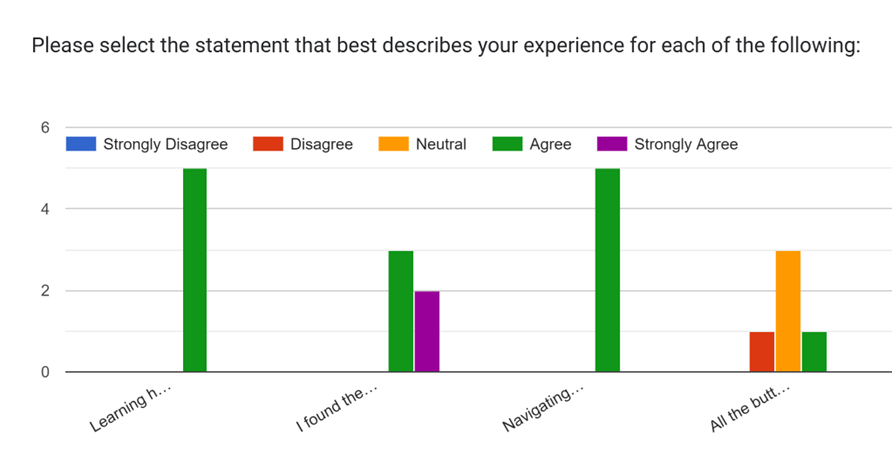
\includegraphics[width=1\textwidth]{images/UsabilityTestResults_pt1.png}
  \caption{Results of Usability Survey - 1}
\end{figure}

\begin{figure}[h]
  \centering
  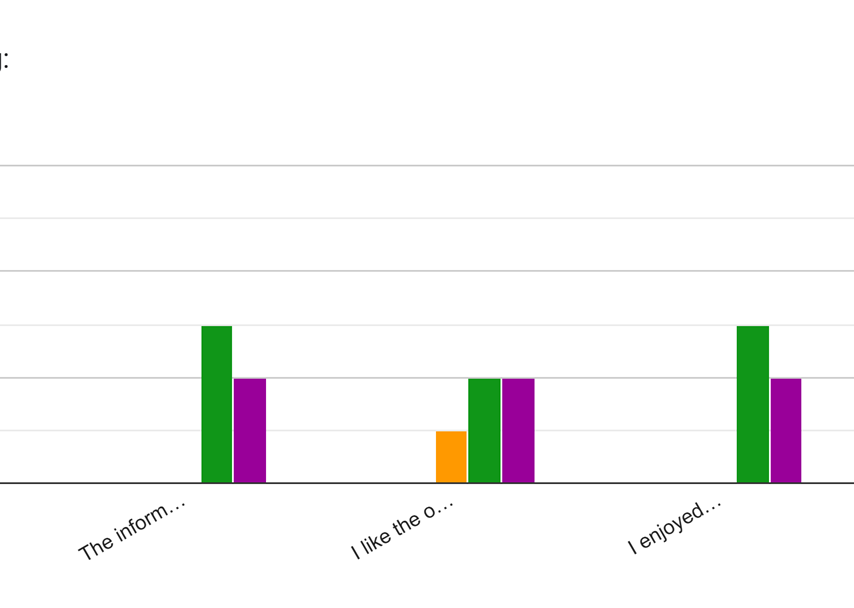
\includegraphics[width=1\textwidth]{images/UsabilityTestResults_pt2.png}
  \caption{Results of Usability Survey - 2}
\end{figure}

\newpage

\begin{mdframed}[linewidth=0.5mm] \par
  \textbf{Test Case Identifier:} UH-ST-PI1 \par
  \textbf{Input:} List of available languages to perform assessments in is available to be selected and listed \par
  \textbf{Expected Output:} The expected result is the available languages for the assessment are English and Mandarin  \par
  \textbf{Actual Output:} The assessment can be completed in either English and Mandarin (Figure 3)\par
  \textbf{Expected and Actual Output Match:} True \par
  \textbf{Relevant Nonfunctional Requirement(s):} UH-PI1
\end{mdframed}

\begin{figure}[h]
  \centering
  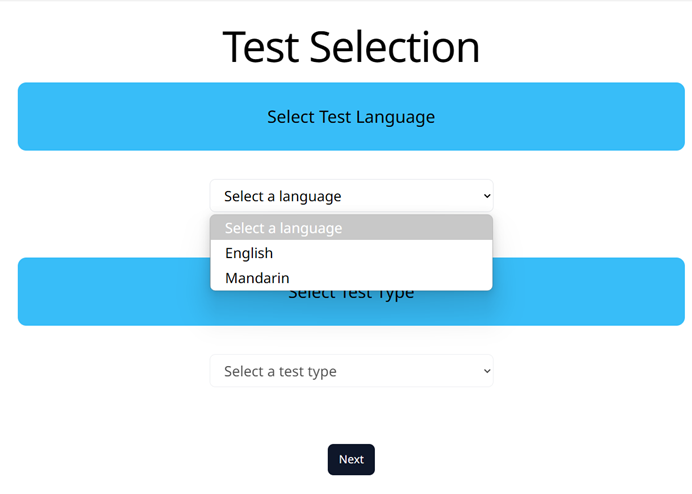
\includegraphics[width=0.8\textwidth]{images/LanguageSelection.png}
  \caption{Language Selection}
\end{figure}

\begin{mdframed}[linewidth=0.5mm] \par
  \textbf{Test Case Identifier:} UH-ST-LI1 \par
  \textbf{Input:} Link to documentation is available on the system's frontend interface, and can be accessed \par
  \textbf{Expected Output:} The expected result is a user can verify the link takes them to access documentation  \par
  \textbf{Actual Output:} No user documentation is linked to the current version of the system\par
  \textbf{Expected and Actual Output Match:} False \par
  \textbf{Relevant Nonfunctional Requirement(s):} UH-LI2
\end{mdframed}

\subsection{Performance}
\hspace{2em}The test cases outlined below ensure proper performance and stability of our system and database.
\begin{mdframed}[linewidth=0.5mm]
  \textbf{Test Case Identifier:} PR-ST-SL1 \par
  \textbf{Input/Condition:} User navigates through various web pages. \par
  \textbf{Expected Output/Results:} All web pages load completely with all functionalities within MAX\_LOAD\_TIME. \par
  \textbf{Actual Output/Results:} All web pages load with correct data within MAX\_LOAD\_TIME. \par
  \textbf{Expected and Actual Output Match:} True \par
  \textbf{Relevant Functional Requirement(s):} PR-ST-SL1
\end{mdframed}

\begin{mdframed}[linewidth=0.5mm]
  \textbf{Test Case Identifier:} PR-ST-SL2 \par
  \textbf{Input/Condition:} A session is recorded during which two faces appear and a keyword is said. \par
  \textbf{Expected Output/Results:} The latency between video and recorded playback remains below SHORT\_PROCESSING\_TIME. \par
  \textbf{Actual Output/Results:} The latency is within the \\SHORT\_PROCESSING\_TIME when reviewing on clinician side \par
  \textbf{Expected and Actual Output Match:} True \par
  \textbf{Relevant Functional Requirement(s):} PR-ST-SL2
\end{mdframed}

\begin{mdframed}[linewidth=0.5mm]
  \textbf{Test Case Identifier:} PR-ST-SL3 \par
  \textbf{Input/Condition:} A video recorded during an assessment session is stored and later retrieved. \par
  \textbf{Expected Output/Results:} The retrieved video meets or exceeds AVERAGE\_RESOLUTION. \par
  \textbf{Actual Output/Results:} Video is AVERAGE\_RESOLUTION\par
  \textbf{Expected and Actual Output Match:} True \par
  \textbf{Relevant Functional Requirement(s):} PR-ST-SL3
\end{mdframed}

\begin{mdframed}[linewidth=0.5mm]
  \textbf{Test Case Identifier:} PR-ST-PA1\par
  \textbf{Input/Condition:} Analysis model loaded with sample audio and video data containing known speech disturbances and multiple faces. \par
  \textbf{Expected Output/Results:} The model detects speech and multiple faces with an accuracy of VERY\_HIGH\_SUCCESS\_RATE. \par
  \textbf{Actual Output/Results:} The model detects multiple faces with \\VERY\_HIGH\_SUCCESS\_RATE but not speeches \par
  \textbf{Expected and Actual Output Match:} False \par
  \textbf{Relevant Functional Requirement(s):} PR-ST-PA1
\end{mdframed}

\begin{mdframed}[linewidth=0.5mm]
  \textbf{Test Case Identifier:} PR-ST-PA3 \par
  \textbf{Input/Condition:} User performs actions in the recorded session \par
  \textbf{Expected Output/Results:} The timestamps delay within \\SHORT\_PROCESSING\_TIME of the real-time action. \par
  \textbf{Actual Output/Results:} The timestamps delay \\SHORT\_PROCESSING\_TIME  \par
  \textbf{Expected and Actual Output Match:} True \par
  \textbf{Relevant Functional Requirement(s):} PR-ST-PA3
\end{mdframed}

\begin{mdframed}[linewidth=0.5mm]
  \textbf{Test Case Identifier:} PR-ST-PA4 \par
  \textbf{Input/Condition:} Manual verification of the answer key’s accuracy. \par
  \textbf{Expected Output/Results:} The expected output is that the answer key is \\MAX\_SUCCESS\_RATE. \par
  \textbf{Actual Output/Results:} The answer key is MAX\_SUCCESS\_RATE.  \par
  \textbf{Expected and Actual Output Match:} True \par
  \textbf{Relevant Functional Requirement(s):} PR-ST-PA4
\end{mdframed}

\begin{mdframed}[linewidth=0.5mm]
  \textbf{Test Case Identifier:} PR-ST-RFT1 \par
  \textbf{Input/Condition:} Simulate common user errors (e.g., invalid inputs). \par
  \textbf{Expected Output/Results:} The system displays clear error messages for at least VERY\_HIGH\_SUCCESS\_RATE of the errors encountered. \par
  \textbf{Actual Output/Results:} System gives correct feedback to user with a VERY\_HIGH\_SUCCESS\_RATE \par
  \textbf{Expected and Actual Output Match:} True \par
  \textbf{Relevant Functional Requirement(s):} PR-ST-RFT1
\end{mdframed}

\begin{mdframed}[linewidth=0.5mm]
  \textbf{Test Case Identifier:} PR-ST-RFT2 \par
  \textbf{Input/Condition:} Monthly data backup event. \par
  \textbf{Expected Output/Results:} The expected output is that the system performs a data backup within a MONTHLY\_BACKUP timeframe on the first of each month. \par
  \textbf{Actual Output/Results:} This test case is currently out of scope as we don't have enough data to verify it.\par
  \textbf{Expected and Actual Output Match:} N/A \par
  \textbf{Relevant Functional Requirement(s):} PR-ST-RFT2
\end{mdframed}

\begin{mdframed}[linewidth=0.5mm]
  \textbf{Test Case Identifier:} PR-ST-CR1 \par
  \textbf{Input/Condition:} System loaded with MIN\_USERS accounts. \par
  \textbf{Expected Output/Results:} The expected result is that the system operates stably and manages all accounts without issues. \par
  \textbf{Actual Output/Results:} System runs smoothly with MIN\_USERS accounts\par
  \textbf{Expected and Actual Output Match:} True \par
  \textbf{Relevant Functional Requirement(s):} PR-ST-CR1
\end{mdframed}

\begin{mdframed}[linewidth=0.5mm]
  \textbf{Test Case Identifier:} PR-ST-CR2 \par
  \textbf{Input/Condition:} Data stored in the database approaches the annual MIN\_STORAGE threshold. \par
  \textbf{Expected Output/Results:} The system accommodates the data volume without performance degradation. \par
  \textbf{Actual Output/Results:} The system accommodates the \\MIN\_STORAGE threshold with room to increase data storage\par
  \textbf{Expected and Actual Output Match:} True \par
  \textbf{Relevant Functional Requirement(s):} PR-ST-CR2
\end{mdframed}

\begin{mdframed}[linewidth=0.5mm]
  \textbf{Test Case Identifier:} PR-ST-SE1 \par
  \textbf{Input/Condition:} Increase user base by \\YEARLY\_INCREASE\_PERCENTAGE. \par
  \textbf{Expected Output/Results:} The expected result is that the system maintains performance while handling user growth. \par
  \textbf{Actual Output/Results:} This test case is currently out of scope due to time constraints\par
  \textbf{Expected and Actual Output Match:} N/A \par
  \textbf{Relevant Functional Requirement(s):} PR-ST-SE1
\end{mdframed}

\begin{mdframed}[linewidth=0.5mm]
  \textbf{Test Case Identifier:} PR-ST-LR1 \par
  \textbf{Input/Condition:} Monitor system stability over successive updates on the release build. \par
  \textbf{Expected Output/Results:} The system’s failure rate remains below LOW\_FAILURE\_RATE during updates. \par
  \textbf{Actual Output/Results:} system failure rate remains below \\LOW\_FAILURE\_RATE during deployment of versions \par
  \textbf{Expected and Actual Output Match:} True \par
  \textbf{Relevant Functional Requirement(s):} PR-ST-LR1
\end{mdframed}

\begin{mdframed}[linewidth=0.5mm]
  \textbf{Test Case Identifier:} PR-ST-LR2 \par
  \textbf{Input/Condition:} The system is run on multiple operating systems (Windows, macOS). \par
  \textbf{Expected Output/Results:} The system functions correctly on all tested platforms without issues. \par
  \textbf{Actual Output/Results:} The system functions correctly on multiple operating systems\par
  \textbf{Expected and Actual Output Match:} True \par
  \textbf{Relevant Functional Requirement(s):} PR-ST-LR2
\end{mdframed}


\subsection{Operational and Environmental}
\hspace{2em}The test results below ensures that the system can be used in a variety of environments,
along with the requirements for which users are expected to use the system within, and the
capabilities and qualities the system has to interact with adjacent systems in the environment.

\begin{mdframed}[linewidth=0.5mm] \par
  \textbf{Test Case Identifier:} OE-ST-EPE1 \par
  \textbf{Input:} Testing the system, including the assessment, on a variety of screen sizes \par
  \textbf{Expected Output:} The expected result is the system's displayed elements will scale appropriately to different screen sizes \par
  \textbf{Actual Output:} The actual result is the system's displayed elements scaled, to the satisfaction of 60\% of users (Figure 4)\par
  \textbf{Expected and Actual Output Match:} True \par
  \textbf{Relevant Nonfunctional Requirement(s):} OE-EPE1
\end{mdframed}

\newpage

\begin{figure}[h]
  \centering
  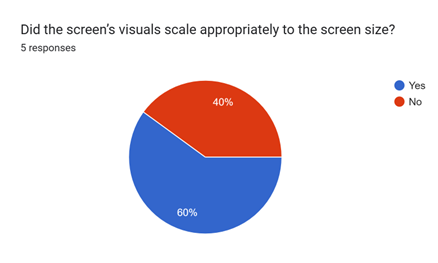
\includegraphics[width=0.8\textwidth]{images/UsabilityTestResults2.png}
  \caption{Results of Usability Survey - Scalability}
\end{figure}

\begin{mdframed}[linewidth=0.5mm] \par
  \textbf{Test Case Identifier:} OE-ST-WE1 \par
  \textbf{Input:} User attempts to start system setup \par
  \textbf{Expected Output:} The expected result is device verification displayed on-screen, informing the user that the environment they're in is suitable for the assessment \par
  \textbf{Actual Output:} The actual result is the system verifies the user can proceed to the assessment following system setup, and allowing the user to test out their peripherals prior to starting the assessment (Figure 5)\par
  \textbf{Expected and Actual Output Match:} True \par
  \textbf{Relevant Nonfunctional Requirement(s):} OE-WE1, OE-WE2
\end{mdframed}

\newpage

\begin{figure}[h]
  \centering
  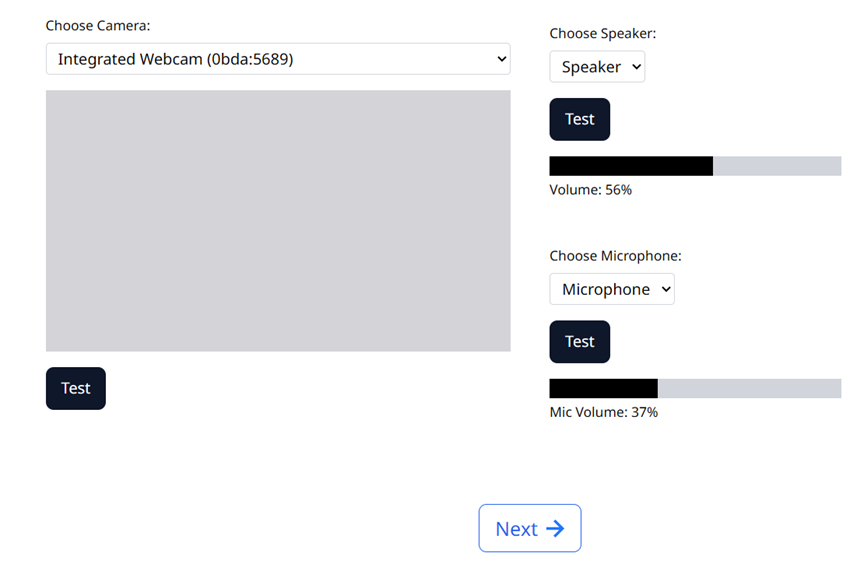
\includegraphics[width=0.8\textwidth]{images/DeviceSetup.png}
  \caption{Device Setup}
\end{figure}

\begin{mdframed}[linewidth=0.5mm] \par
  \textbf{Test Case Identifier:} OE-ST-IA1 \par
  \textbf{Input:} Assessment is complete, and results need to be stored \par
  \textbf{Expected Output:} Verify results are stored in the external server \par
  \textbf{Actual Output:} Results can be accessed through the server to ensure data has been uploaded and stored successful (Figure 6 and Figure 7)\par
  \textbf{Expected and Actual Output Match:} True \par
  \textbf{Relevant Nonfunctional Requirement(s):} OE-IA1
\end{mdframed}

\begin{figure}[p]
  \centering
  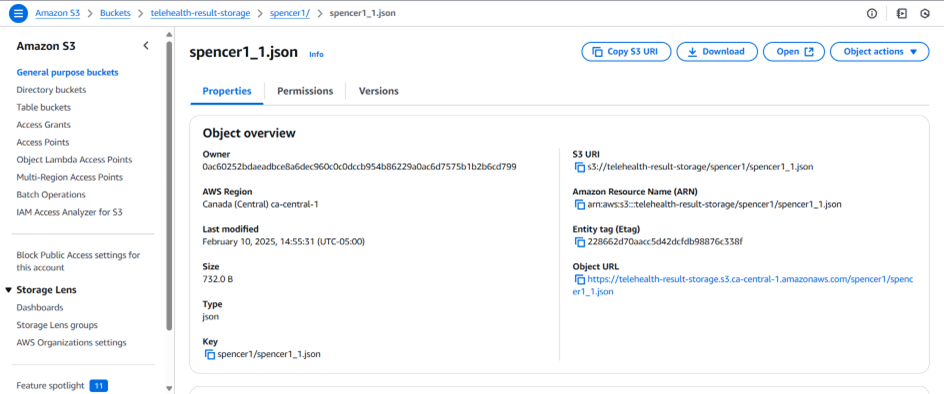
\includegraphics[width=0.8\textwidth]{images/ResultsStorage.png}
  \caption{Results Storage - AWS}
\end{figure}

\begin{figure}[p]
  \centering
  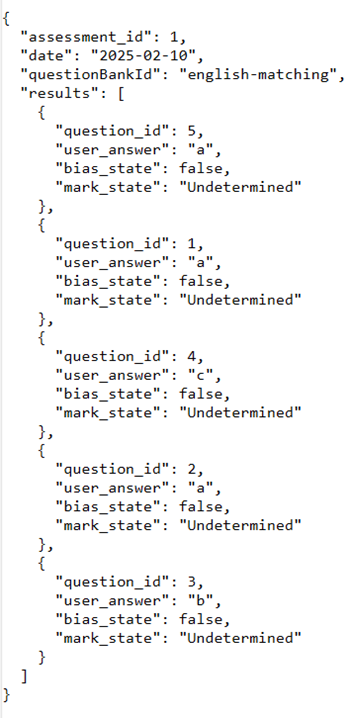
\includegraphics[width=0.5\textwidth]{images/ResultsStorage2.png}
  \caption{Results Storage - JSON}
\end{figure}

\clearpage

\subsection{Maintainability and Support}
\hspace{2em}These test cases ensure the platform meets its maintenance, support, and adaptability requirements effectively.

\begin{mdframed}[linewidth=0.5mm] \par
  \textbf{Test Case Identifier:} MS-ST-MSA1 \par
  \textbf{Input:} Perform updates to individual components and simulate user feedback submissions via the GitHub repository. \par
  \textbf{Expected Output:} The expected result is that each component update does not exceed \\NUM\_CODE\_LINES lines of code edited outside the updated module, and users can submit issues and feature requests directly to GitHub, categorized as issues, feature requests, or feedback. \par
  \textbf{Actual Output:} The actual result is that each component update does not exceed \\NUM\_CODE\_LINES lines of code edited outside the updated module, and users can submit issues and feature requests directly to GitHub, categorized as issues, feature requests, or feedback. \par
  \textbf{Expected and Actual Output Match:} True \par
  \textbf{Relevant Nonfunctional Requirement(s):} MS-MR1, MS-SR1
\end{mdframed}

\begin{figure}[h]
  \centering
  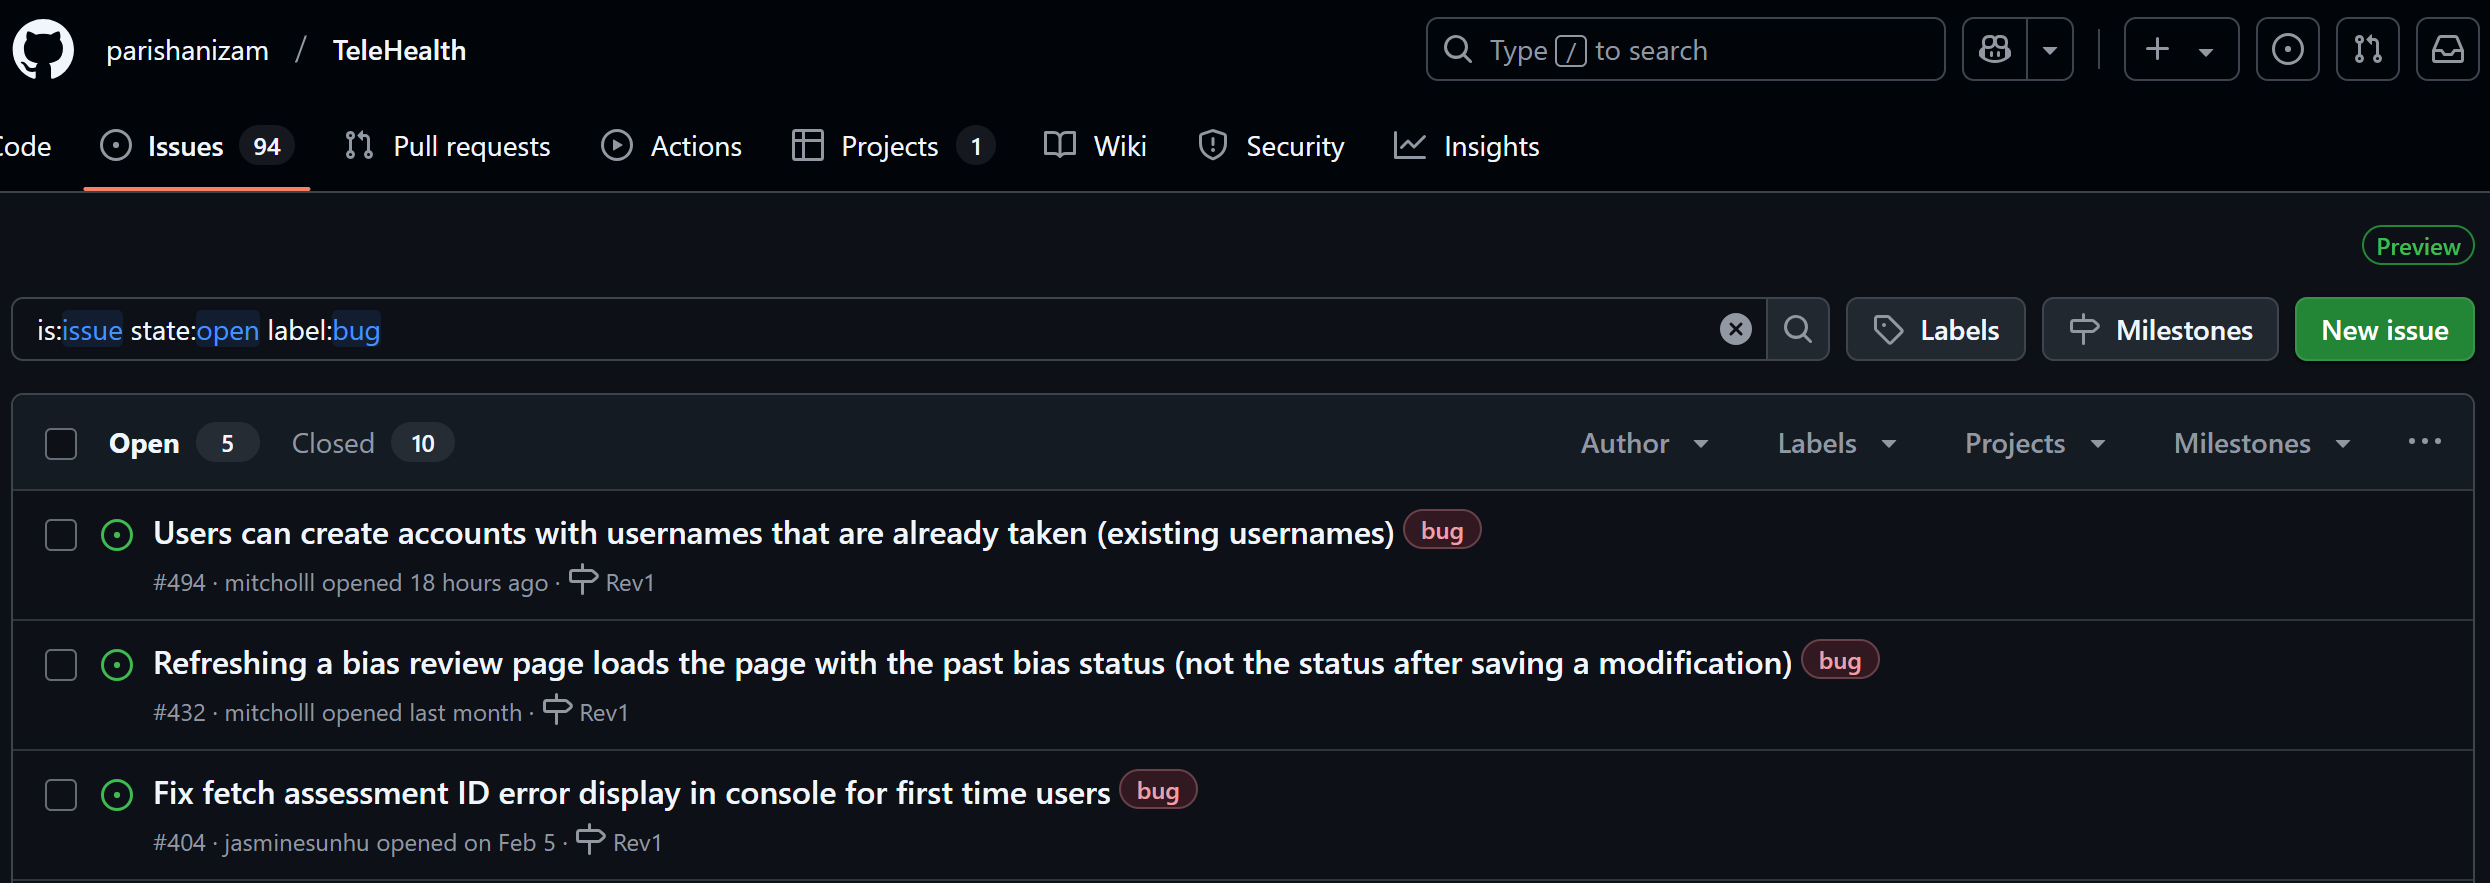
\includegraphics[width=1\textwidth]{images/MS-ST-MSA1.png}
  \caption{GitHub Issue Creation}
\end{figure}

\begin{mdframed}[linewidth=0.5mm] \par
  \textbf{Test Case Identifier:} MS-ST-MSA2 \par
  \textbf{Input:} New user group follows the tutorial to complete primary tasks (e.g., starting an assessment). \par
  \textbf{Expected Output:} The expected result is HIGH\_SUCCESS\_RATE of users can complete core tasks \\correctly after following the tutorial. \par
  \textbf{Actual Output:} The actual result is HIGH\_SUCCESS\_RATE of users can complete core tasks \\correctly after following the tutorial. \par
  \textbf{Expected and Actual Output Match:} True \par
  \textbf{Relevant Nonfunctional Requirement(s):} MS-SR2
\end{mdframed}

\begin{mdframed}[linewidth=0.5mm] \par
  \textbf{Test Case Identifier:} MS-ST-MSA3 \par
  \textbf{Input:} Load and navigate the platform across multiple devices to evaluate responsive design and functionality. \par
  \textbf{Expected Output:} The expected result is MAX\_SUCCESS\_RATE of essential features are fully functional and readable across all screen sizes tested. \par
  \textbf{Actual Output:} The actual result is MAX\_SUCCESS\_RATE of essential features are fully \\functional and readable across all screen sizes tested. \par
  \textbf{Expected and Actual Output Match:} True \par
  \textbf{Relevant Nonfunctional Requirement(s):} MS-AR1
\end{mdframed}

\begin{figure}[p]
  \centering
  
\includegraphics[width=0.75\textwidth]{images/TIscreensizeIpad.png}
  \caption{Website on iPad Screen Size}
\end{figure}

\begin{figure}[p]
  \centering
  
\includegraphics[width=0.5\textwidth]{images/TIscreensizeIphone.png}
  \caption{Website on iPhone Screen Size}
\end{figure}

\begin{figure}[p]
  \centering
  
\includegraphics[width=1\textwidth]{images/TIscreensizeSurface.png}
  \caption{Website on Surface Laptop Screen Size}
\end{figure}

\clearpage

\subsection{Cultural}
\hspace{2em}These tests ensure that the platform respects cultural sensitivities and provides full bilingual support, enhancing inclusiveness and accessibility for diverse user groups.

\begin{mdframed}[linewidth=0.5mm] \par
  \textbf{Test Case Identifier:} CU-ST-CUR1 \par
  \textbf{Input:} User acceptance testing gathers feedback from a diverse set of users. \par
  \textbf{Expected Output:} The expected result is MAX\_SUCESS\_RATE of reviewed content is confirmed as culturally sensitive with no instances of offensive language or imagery. \par
  \textbf{Actual Output:} The actual result is MAX\_SUCESS\_RATE of reviewed content is confirmed as culturally sensitive with no instances of offensive language or imagery. \par
  \textbf{Expected and Actual Output Match:} True \par
  \textbf{Relevant Nonfunctional Requirement(s):} CU-CR1
\end{mdframed}

\begin{mdframed}[linewidth=0.5mm] \par
  \textbf{Test Case Identifier:} CU-ST-CUR2 \par
  \textbf{Input:} Platform is available in both English and Mandarin, with all interface elements and assessments translated. \par
  \textbf{Expected Output:} The expected result is MAX\_SUCCESS\_RATE of assessment content is fully \\translated and functional in both English and Mandarin with no \\untranslated elements. \par
  \textbf{Actual Output:} The actual result is MAX\_SUCCESS\_RATE of assessment content is fully \\translated and functional in English, but only the assessment itself is also available in Mandarin. \par
  \textbf{Expected and Actual Output Match:} False \par
  \textbf{Relevant Nonfunctional Requirement(s):} CU-CR2
\end{mdframed}

\subsection{Security}
\hspace{2em}The test cases below 

\begin{mdframed}[linewidth=0.5mm] \par
  \textbf{Test Case Identifier:} FR-ST-A1 \par
  \textbf{Input:} Selection of Parent account role for login \par
  \textbf{Expected Output:} The expected result is the Parent account role is selected and User is brought to the Parent login screen \par
  \textbf{Actual Output:} \par
  \textbf{Expected and Actual Output Match:} True \par
  \textbf{Relevant Nonfunctional Requirement(s):} FR-A1
\end{mdframed}

\subsection{Compliance}
\hspace{2em}The test cases below 

\begin{mdframed}[linewidth=0.5mm] \par
  \textbf{Test Case Identifier:} FR-ST-A1 \par
  \textbf{Input:} Selection of Parent account role for login \par
  \textbf{Expected Output:} The expected result is the Parent account role is selected and User is brought to the Parent login screen \par
  \textbf{Actual Output:} \par
  \textbf{Expected and Actual Output Match:} True \par
  \textbf{Relevant Nonfunctional Requirement(s):} FR-A1
\end{mdframed}
	
\section{Comparison to Existing Implementation}	

As this project does not have existing implementations, this section is not appropriate for the TeleHealth Insights project.

\section{Unit Testing}

\section{Changes Due to Testing}

\hspace{2em} Throughout testing, important changes to the system were identified that will be implemented into Revision 1.
Feedback is based on pilot usability testing with fellow software engineering students, graduates from McMaster, and the team's
supervisor, following the Revision 0 demo. The changes identiifed are aimed at enhancing the functionality and usability of the system.

\begin{itemize}
  \item \textbf{Parent Results Accessibility} Inititally, the system was not capable of displaying the results to the parents. Upon conversations
    with the team's supervisor, it became clear that a missing feature that would benefit users of the system is for parents to have access to
    their own past assessment information. Clarity in communication surrounding their child's results is integral for conversation amongst
    parents and clinicians to see how the child's progress overtime.
  \item \textbf{Uploading Results Require Clearer Communication} Initially, to upload results, the user would press a 'submit' button on the last question
    of their assessment. Upon clicking this button, text would appear to inform the user that their results were being uploaded. However, feedback from
    the team's usability testing revealed that users would appreciate a loading screen, or a loading indicator on the screen, rather than static text
    to effectively communicate that results are still being uploaded. Users were previously confused on whether or not the system was operating properly,
    or if it froze, due to the lack of a loading indicator.
  \item \textbf{Simplify Tutorials} The tutorial screens consisted of a variety of screenshots and descriptions, informing users of what they could expect
    to see from the system upon completion of the tutorial. However, upon conducting usability testing, numerous users were confused by the tutorial,
    and thought that the screenshots themselves were interactable buttons, as they were screenshots of the system. Tutorials will be modified to convey
    integral information to the user about the assessment itself, and minimize repetition of information by reducing screenshots of the system. The section
    of the tutorial users appreciated was the step-by-step walkthrough of a sample question. The tutorial will be reformulated to put a larger emphasis on
    walking users through the system, instead of displaying static information.
  \item \textbf{Uploading Assessment Videos} The team's supervisor expressed through feedback that the system was not effective at uploading assessment videos.
    Upon inspection, the team updated the deployed system to allow for faster upload speeds, resulting in a better user experience when completing assessments.
    This is of particular importance to the team, as the full assessment will be 30 questions, while the usability test featured only 5 questions. In addition,
    the system will be used by children, which may lengthen the assessment duration as well.
\end{itemize}

\section{Automated Testing}

\subsection{Linters}
To maintain a good coding standard, we integrated linters into
our development workflow. For JavaScript files, we rely on Prettier to
automatically format code, ensuring consistent indentation and spacing.
By running Prettier as part of our pre-commit checks, any formatting concerns
are addressed before merging into our main repository, which helps minimize merge
conflicts and maintain a clean codebase.

\subsection{Unit Testing}
We use Jest as our primary JavaScript testing framework to automatically verify critical parts 
of our code before changes are merged into the main branch. This approach helps us catch issues 
early, maintain code quality, and keep the overall system stable.

\subsection{Continuous Integration}
We used continuous integration (CI) pipeline to automate test execution
and provide immediate feedback whenever new code is committed. We configure GitHub
Actions trigger to run our Jest unit tests, linters and document tests on each pull request 
or direct push to main, ensuring that only code meeting quality standards is always met.


		
\section{Trace to Requirements}

\begin{table}[!ht]
  \caption{Traceability Table Between System Test Cases and Functional Requirements (Part 1)}
  \resizebox{\textwidth}{!}{
  \begin{tabular}{|l|l|l|l|l|l|l|l|l|l|l|l|l|l|l|l|l|}
  \hline
      ~ & FR-ST-A1 & FR-ST-A2 & FR-ST-A3 & FR-ST-A4 & FR-ST-A5 & FR-ST-A6 & FR-ST-A7 & FR-ST-A8 & FR-ST-DSC1 & FR-ST-DSC2 & FR-ST-DSC3 & FR-ST-DSC4 & FR-ST-DSC5 & FR-ST-VDA1 & FR-ST-VDA2 \\ \hline
      FR-A1 & X & X & ~ & ~ & ~ & ~ & ~ & ~ & ~ & ~ & ~ & ~ & ~ & ~ & ~ \\ \hline
      FR-A2 & ~ & ~ & X & X & ~ & ~ & ~ & ~ & ~ & ~ & ~ & ~ & ~ & ~ & ~ \\ \hline
      FR-A3 & ~ & ~ & ~ & ~ & X & X & ~ & ~ & ~ & ~ & ~ & ~ & ~ & ~ & ~ \\ \hline
      FR-A4 & ~ & ~ & ~ & ~ & ~ & ~ & X & ~ & ~ & ~ & ~ & ~ & ~ & ~ & ~ \\ \hline
      FR-A5 & ~ & ~ & ~ & ~ & ~ & ~ & ~ & X & ~ & ~ & ~ & ~ & ~ & ~ & ~ \\ \hline
      FR-SS1 & ~ & ~ & ~ & ~ & ~ & ~ & ~ & ~ & ~ & ~ & ~ & ~ & ~ & ~ & ~ \\ \hline
      FR-SS2 & ~ & ~ & ~ & ~ & ~ & ~ & ~ & ~ & ~ & ~ & ~ & ~ & ~ & ~ & ~ \\ \hline
      FR-SS3 & ~ & ~ & ~ & ~ & ~ & ~ & ~ & ~ & ~ & ~ & ~ & ~ & ~ & ~ & ~ \\ \hline
      FR-SS4 & ~ & ~ & ~ & ~ & ~ & ~ & ~ & ~ & ~ & ~ & ~ & ~ & ~ & ~ & ~ \\ \hline
      FR-SS5 & ~ & ~ & ~ & ~ & ~ & ~ & ~ & ~ & ~ & ~ & ~ & ~ & ~ & ~ & ~ \\ \hline
      FR-AI1 & ~ & ~ & ~ & ~ & ~ & ~ & ~ & ~ & ~ & ~ & ~ & ~ & ~ & ~ & ~ \\ \hline
      FR-AI2 & ~ & ~ & ~ & ~ & ~ & ~ & ~ & ~ & ~ & ~ & ~ & ~ & ~ & ~ & ~ \\ \hline
      FR-AI3 & ~ & ~ & ~ & ~ & ~ & ~ & ~ & ~ & ~ & ~ & ~ & ~ & ~ & ~ & ~ \\ \hline
      FR-AI4 & ~ & ~ & ~ & ~ & ~ & ~ & ~ & ~ & ~ & ~ & ~ & ~ & ~ & ~ & ~ \\ \hline
      FR-AI5 & ~ & ~ & ~ & ~ & ~ & ~ & ~ & ~ & ~ & ~ & ~ & ~ & ~ & ~ & ~ \\ \hline
      FR-AI6 & ~ & ~ & ~ & ~ & ~ & ~ & ~ & ~ & ~ & ~ & ~ & ~ & ~ & ~ & ~ \\ \hline
      FR-AI7 & ~ & ~ & ~ & ~ & ~ & ~ & ~ & ~ & ~ & ~ & ~ & ~ & ~ & ~ & ~ \\ \hline
      FR-DSC1 & ~ & ~ & ~ & ~ & ~ & ~ & ~ & ~ & X & ~ & ~ & ~ & ~ & ~ & ~ \\ \hline
      FR-DSC2 & ~ & ~ & ~ & ~ & ~ & ~ & ~ & ~ & ~ & X & ~ & ~ & ~ & ~ & ~ \\ \hline
      FR-DSC3 & ~ & ~ & ~ & ~ & ~ & ~ & ~ & ~ & ~ & ~ & X & ~ & ~ & ~ & ~ \\ \hline
      FR-DSC4 & ~ & ~ & ~ & ~ & ~ & ~ & ~ & ~ & ~ & ~ & ~ & X & ~ & ~ & ~ \\ \hline
      FR-DSC5 & ~ & ~ & ~ & ~ & ~ & ~ & ~ & ~ & ~ & ~ & ~ & ~ & X & ~ & ~ \\ \hline
      FR-VADA1 & ~ & ~ & ~ & ~ & ~ & ~ & ~ & ~ & ~ & ~ & ~ & ~ & ~ & X & ~ \\ \hline
      FR-VADA2 & ~ & ~ & ~ & ~ & ~ & ~ & ~ & ~ & ~ & ~ & ~ & ~ & ~ & ~ & X \\ \hline
      FR-VADA3 & ~ & ~ & ~ & ~ & ~ & ~ & ~ & ~ & ~ & ~ & ~ & ~ & ~ & ~ & ~ \\ \hline
      FR-DPD1 & ~ & ~ & ~ & ~ & ~ & ~ & ~ & ~ & ~ & ~ & ~ & ~ & ~ & ~ & ~ \\ \hline
      FR-DPD2 & ~ & ~ & ~ & ~ & ~ & ~ & ~ & ~ & ~ & ~ & ~ & ~ & ~ & ~ & ~ \\ \hline
      FR-DPD3 & ~ & ~ & ~ & ~ & ~ & ~ & ~ & ~ & ~ & ~ & ~ & ~ & ~ & ~ & ~ \\ \hline
      FR-DPD4 & ~ & ~ & ~ & ~ & ~ & ~ & ~ & ~ & ~ & ~ & ~ & ~ & ~ & ~ & ~ \\ \hline
  \end{tabular}
  }
\end{table}

\begin{table}[!ht]
  \caption{Traceability Table Between System Test Cases and Functional Requirements (Part 2)}
  \resizebox{\textwidth}{!}{
  \begin{tabular}{|l|l|l|l|l|l|l|l|l|l|l|l|l|l|l|l|l|l|}
  \hline
      ~ & FR-ST-VDA3 & FR-ST-DPD1 & FR-ST-DPD2 & FR-ST-DPD3 & FR-ST-DPD4 & FR-ST-SS1 & FR-ST-SS2 & FR-ST-SS3 & FR-ST-SS4 & FR-ST-SS5 & FR-ST-AI1 & FR-ST-AI2 & FR-ST-AI3 & FR-ST-AI4 & FR-ST-AI5 & FR-ST-AI6 & FR-ST-AI7 \\ \hline
      FR-A1 & ~ & ~ & ~ & ~ & ~ & ~ & ~ & ~ & ~ & ~ & ~ & ~ & ~ & ~ & ~ & ~ & ~ \\ \hline
      FR-A2 & ~ & ~ & ~ & ~ & ~ & ~ & ~ & ~ & ~ & ~ & ~ & ~ & ~ & ~ & ~ & ~ & ~ \\ \hline
      FR-A3 & ~ & ~ & ~ & ~ & ~ & ~ & ~ & ~ & ~ & ~ & ~ & ~ & ~ & ~ & ~ & ~ & ~ \\ \hline
      FR-A4 & ~ & ~ & ~ & ~ & ~ & ~ & ~ & ~ & ~ & ~ & ~ & ~ & ~ & ~ & ~ & ~ & ~ \\ \hline
      FR-A5 & ~ & ~ & ~ & ~ & ~ & ~ & ~ & ~ & ~ & ~ & ~ & ~ & ~ & ~ & ~ & ~ & ~ \\ \hline
      FR-SS1 & ~ & ~ & ~ & ~ & ~ & X & ~ & ~ & ~ & ~ & ~ & ~ & ~ & ~ & ~ & ~ & ~ \\ \hline
      FR-SS2 & ~ & ~ & ~ & ~ & ~ & ~ & X & ~ & ~ & ~ & ~ & ~ & ~ & ~ & ~ & ~ & ~ \\ \hline
      FR-SS3 & ~ & ~ & ~ & ~ & ~ & ~ & ~ & X & ~ & ~ & ~ & ~ & ~ & ~ & ~ & ~ & ~ \\ \hline
      FR-SS4 & ~ & ~ & ~ & ~ & ~ & ~ & ~ & ~ & X & ~ & ~ & ~ & ~ & ~ & ~ & ~ & ~ \\ \hline
      FR-SS5 & ~ & ~ & ~ & ~ & ~ & ~ & ~ & ~ & ~ & X & ~ & ~ & ~ & ~ & ~ & ~ & ~ \\ \hline
      FR-AI1 & ~ & ~ & ~ & ~ & ~ & ~ & ~ & ~ & ~ & ~ & X & ~ & ~ & ~ & ~ & ~ & ~ \\ \hline
      FR-AI2 & ~ & ~ & ~ & ~ & ~ & ~ & ~ & ~ & ~ & ~ & ~ & X & ~ & ~ & ~ & ~ & ~ \\ \hline
      FR-AI3 & ~ & ~ & ~ & ~ & ~ & ~ & ~ & ~ & ~ & ~ & ~ & ~ & X & ~ & ~ & ~ & ~ \\ \hline
      FR-AI4 & ~ & ~ & ~ & ~ & ~ & ~ & ~ & ~ & ~ & ~ & ~ & ~ & ~ & X & ~ & ~ & ~ \\ \hline
      FR-AI5 & ~ & ~ & ~ & ~ & ~ & ~ & ~ & ~ & ~ & ~ & ~ & ~ & ~ & ~ & X & ~ & ~ \\ \hline
      FR-AI6 & ~ & ~ & ~ & ~ & ~ & ~ & ~ & ~ & ~ & ~ & ~ & ~ & ~ & ~ & ~ & X & ~ \\ \hline
      FR-AI7 & ~ & ~ & ~ & ~ & ~ & ~ & ~ & ~ & ~ & ~ & ~ & ~ & ~ & ~ & ~ & ~ & X \\ \hline
      FR-DSC1 & ~ & ~ & ~ & ~ & ~ & ~ & ~ & ~ & ~ & ~ & ~ & ~ & ~ & ~ & ~ & ~ & ~ \\ \hline
      FR-DSC2 & ~ & ~ & ~ & ~ & ~ & ~ & ~ & ~ & ~ & ~ & ~ & ~ & ~ & ~ & ~ & ~ & ~ \\ \hline
      FR-DSC3 & ~ & ~ & ~ & ~ & ~ & ~ & ~ & ~ & ~ & ~ & ~ & ~ & ~ & ~ & ~ & ~ & ~ \\ \hline
      FR-DSC4 & ~ & ~ & ~ & ~ & ~ & ~ & ~ & ~ & ~ & ~ & ~ & ~ & ~ & ~ & ~ & ~ & ~ \\ \hline
      FR-DSC5 & ~ & ~ & ~ & ~ & ~ & ~ & ~ & ~ & ~ & ~ & ~ & ~ & ~ & ~ & ~ & ~ & ~ \\ \hline
      FR-VADA1 & ~ & ~ & ~ & ~ & ~ & ~ & ~ & ~ & ~ & ~ & ~ & ~ & ~ & ~ & ~ & ~ & ~ \\ \hline
      FR-VADA2 & ~ & ~ & ~ & ~ & ~ & ~ & ~ & ~ & ~ & ~ & ~ & ~ & ~ & ~ & ~ & ~ & ~ \\ \hline
      FR-VADA3 & X & ~ & ~ & ~ & ~ & ~ & ~ & ~ & ~ & ~ & ~ & ~ & ~ & ~ & ~ & ~ & ~ \\ \hline
      FR-DPD1 & ~ & X & ~ & ~ & ~ & ~ & ~ & ~ & ~ & ~ & ~ & ~ & ~ & ~ & ~ & ~ & ~ \\ \hline
      FR-DPD2 & ~ & ~ & X & ~ & ~ & ~ & ~ & ~ & ~ & ~ & ~ & ~ & ~ & ~ & ~ & ~ & ~ \\ \hline
      FR-DPD3 & ~ & ~ & ~ & X & ~ & ~ & ~ & ~ & ~ & ~ & ~ & ~ & ~ & ~ & ~ & ~ & ~ \\ \hline
      FR-DPD4 & ~ & ~ & ~ & ~ & X & ~ & ~ & ~ & ~ & ~ & ~ & ~ & ~ & ~ & ~ & ~ & ~ \\ \hline
  \end{tabular}
  }
\end{table}

\begin{table}[!ht]
  \caption{Traceability Table Between System Test Cases and Nonfunctional Requirements (Part 1)}
  \resizebox{\textwidth}{!}{
  \begin{tabular}{|l|l|l|l|l|l|l|l|l|l|l|l|l|l|l|l|l|l|}
  \hline
      ~ & LF-ST-LFR1 & LF-ST-LFR2 & UH-ST-EOU1 & UH-ST-PI1 & UH-ST-LI2 & PR-ST-SL1 & PR-ST-SL2 & PR-ST-SL3 & PR-ST-PA1 & PR-ST-PA3 & PR-ST-PA4 & PR-ST-RFT1 & PR-ST-RFT2 & PR-ST-CR1 & PR-ST-CR2 & PR-ST-SE1 & PR-ST-LR1 \\ \hline
      LF-AR1 & X & ~ & ~ & ~ & ~ & ~ & ~ & ~ & ~ & ~ & ~ & ~ & ~ & ~ & ~ & ~ & ~ \\ \hline
      LF-AR2 & X & ~ & ~ & ~ & ~ & ~ & ~ & ~ & ~ & ~ & ~ & ~ & ~ & ~ & ~ & ~ & ~ \\ \hline
      LF-AR3 & ~ & X & ~ & ~ & ~ & ~ & ~ & ~ & ~ & ~ & ~ & ~ & ~ & ~ & ~ & ~ & ~ \\ \hline
      LF-AR4 & X & ~ & ~ & ~ & ~ & ~ & ~ & ~ & ~ & ~ & ~ & ~ & ~ & ~ & ~ & ~ & ~ \\ \hline
      LF-AR5 & ~ & X & ~ & ~ & ~ & ~ & ~ & ~ & ~ & ~ & ~ & ~ & ~ & ~ & ~ & ~ & ~ \\ \hline
      LF-SR1 & ~ & X & ~ & ~ & ~ & ~ & ~ & ~ & ~ & ~ & ~ & ~ & ~ & ~ & ~ & ~ & ~ \\ \hline
      LF-SR2 & ~ & X & ~ & ~ & ~ & ~ & ~ & ~ & ~ & ~ & ~ & ~ & ~ & ~ & ~ & ~ & ~ \\ \hline
      UH-EOU1 & ~ & ~ & X & ~ & ~ & ~ & ~ & ~ & ~ & ~ & ~ & ~ & ~ & ~ & ~ & ~ & ~ \\ \hline
      UH-EOU2 & ~ & ~ & X & ~ & ~ & ~ & ~ & ~ & ~ & ~ & ~ & ~ & ~ & ~ & ~ & ~ & ~ \\ \hline
      UH-PI1 & ~ & ~ & ~ & X & ~ & ~ & ~ & ~ & ~ & ~ & ~ & ~ & ~ & ~ & ~ & ~ & ~ \\ \hline
      UH-LI1 & ~ & ~ & X & ~ & ~ & ~ & ~ & ~ & ~ & ~ & ~ & ~ & ~ & ~ & ~ & ~ & ~ \\ \hline
      UH-LI2 & ~ & ~ & ~ & ~ & X & ~ & ~ & ~ & ~ & ~ & ~ & ~ & ~ & ~ & ~ & ~ & ~ \\ \hline
      UH-UP1 & ~ & ~ & X & ~ & ~ & ~ & ~ & ~ & ~ & ~ & ~ & ~ & ~ & ~ & ~ & ~ & ~ \\ \hline
      UH-AR1 & ~ & ~ & X & ~ & ~ & ~ & ~ & ~ & ~ & ~ & ~ & ~ & ~ & ~ & ~ & ~ & ~ \\ \hline
      PR-SL1 & ~ & ~ & ~ & ~ & ~ & X & ~ & ~ & ~ & ~ & ~ & ~ & ~ & ~ & ~ & ~ & ~ \\ \hline
      PR-SL2 & ~ & ~ & ~ & ~ & ~ & ~ & X & ~ & ~ & ~ & ~ & ~ & ~ & ~ & ~ & ~ & ~ \\ \hline
      PR-SL3 & ~ & ~ & ~ & ~ & ~ & ~ & ~ & X & ~ & ~ & ~ & ~ & ~ & ~ & ~ & ~ & ~ \\ \hline
      PR-SL4 & ~ & ~ & ~ & ~ & ~ & ~ & ~ & ~ & ~ & ~ & ~ & ~ & ~ & ~ & ~ & ~ & ~ \\ \hline
      PR-SCL1 & ~ & ~ & ~ & ~ & ~ & ~ & ~ & ~ & ~ & ~ & ~ & ~ & ~ & ~ & ~ & ~ & ~ \\ \hline
      PR-PA1 & ~ & ~ & ~ & ~ & ~ & ~ & ~ & ~ & X & ~ & ~ & ~ & ~ & ~ & ~ & ~ & ~ \\ \hline
      PR-PA2 & ~ & ~ & ~ & ~ & ~ & ~ & ~ & ~ & X & ~ & ~ & ~ & ~ & ~ & ~ & ~ & ~ \\ \hline
      PR-PA3 & ~ & ~ & ~ & ~ & ~ & ~ & ~ & ~ & ~ & X & ~ & ~ & ~ & ~ & ~ & ~ & ~ \\ \hline
      PR-PA4 & ~ & ~ & ~ & ~ & ~ & ~ & ~ & ~ & ~ & ~ & X & ~ & ~ & ~ & ~ & ~ & ~ \\ \hline
      PR-PA5 & ~ & ~ & ~ & ~ & ~ & ~ & ~ & ~ & ~ & ~ & X & ~ & ~ & ~ & ~ & ~ & ~ \\ \hline
      PR-RFT1 & ~ & ~ & ~ & ~ & ~ & ~ & ~ & ~ & ~ & ~ & ~ & X & ~ & ~ & ~ & ~ & ~ \\ \hline
      PR-RFT2 & ~ & ~ & ~ & ~ & ~ & ~ & ~ & ~ & ~ & ~ & ~ & ~ & X & ~ & ~ & ~ & ~ \\ \hline
      PR-RFT3 & ~ & ~ & ~ & ~ & ~ & ~ & ~ & ~ & ~ & ~ & ~ & X & ~ & ~ & ~ & ~ & ~ \\ \hline
      PR-CR1 & ~ & ~ & ~ & ~ & ~ & ~ & ~ & ~ & ~ & ~ & ~ & ~ & ~ & X & ~ & ~ & ~ \\ \hline
      PR-CR2 & ~ & ~ & ~ & ~ & ~ & ~ & ~ & ~ & ~ & ~ & ~ & ~ & ~ & ~ & X & ~ & ~ \\ \hline
      PR-CR3 & ~ & ~ & ~ & ~ & ~ & ~ & ~ & ~ & ~ & ~ & ~ & ~ & ~ & X & ~ & ~ & ~ \\ \hline
      PR-CR4 & ~ & ~ & ~ & ~ & ~ & ~ & ~ & ~ & ~ & ~ & ~ & ~ & ~ & X & ~ & ~ & ~ \\ \hline
      PR-SE1 & ~ & ~ & ~ & ~ & ~ & ~ & ~ & ~ & ~ & ~ & ~ & ~ & ~ & ~ & ~ & X & ~ \\ \hline
      PR-SE2 & ~ & ~ & ~ & ~ & ~ & ~ & ~ & ~ & ~ & ~ & ~ & ~ & ~ & ~ & X & ~ & ~ \\ \hline
      PR-SE3 & ~ & ~ & ~ & ~ & ~ & ~ & ~ & ~ & ~ & ~ & ~ & ~ & ~ & ~ & X & ~ & ~ \\ \hline
      PR-LR1 & ~ & ~ & ~ & ~ & ~ & ~ & ~ & ~ & ~ & ~ & ~ & ~ & ~ & ~ & ~ & ~ & X \\ \hline
      PR-LR2 & ~ & ~ & ~ & ~ & ~ & ~ & ~ & ~ & ~ & ~ & ~ & ~ & ~ & ~ & ~ & ~ & ~ \\ \hline
      OE-EPE1 & ~ & ~ & ~ & ~ & ~ & ~ & ~ & ~ & ~ & ~ & ~ & ~ & ~ & ~ & ~ & ~ & ~ \\ \hline
      OE-WE1 & ~ & ~ & ~ & ~ & ~ & ~ & ~ & ~ & ~ & ~ & ~ & ~ & ~ & ~ & ~ & ~ & ~ \\ \hline
      OE-WE2 & ~ & ~ & ~ & ~ & ~ & ~ & ~ & ~ & ~ & ~ & ~ & ~ & ~ & ~ & ~ & ~ & ~ \\ \hline
      OE-IA1 & ~ & ~ & ~ & ~ & ~ & ~ & ~ & ~ & ~ & ~ & ~ & ~ & ~ & ~ & ~ & ~ & ~ \\ \hline
      MS-MR1 & ~ & ~ & ~ & ~ & ~ & ~ & ~ & ~ & ~ & ~ & ~ & ~ & ~ & ~ & ~ & ~ & ~ \\ \hline
      MS-SR1 & ~ & ~ & ~ & ~ & ~ & ~ & ~ & ~ & ~ & ~ & ~ & ~ & ~ & ~ & ~ & ~ & ~ \\ \hline
      MS-SR2 & ~ & ~ & ~ & ~ & ~ & ~ & ~ & ~ & ~ & ~ & ~ & ~ & ~ & ~ & ~ & ~ & ~ \\ \hline
      MS-AR1 & ~ & ~ & ~ & ~ & ~ & ~ & ~ & ~ & ~ & ~ & ~ & ~ & ~ & ~ & ~ & ~ & ~ \\ \hline
      SR-AC1 & ~ & ~ & ~ & ~ & ~ & ~ & ~ & ~ & ~ & ~ & ~ & ~ & ~ & ~ & ~ & ~ & ~ \\ \hline
      SR-AC2 & ~ & ~ & ~ & ~ & ~ & ~ & ~ & ~ & ~ & ~ & ~ & ~ & ~ & ~ & ~ & ~ & ~ \\ \hline
      SR-AC3 & ~ & ~ & ~ & ~ & ~ & ~ & ~ & ~ & ~ & ~ & ~ & ~ & ~ & ~ & ~ & ~ & ~ \\ \hline
      SR-AC4 & ~ & ~ & ~ & ~ & ~ & ~ & ~ & ~ & ~ & ~ & ~ & ~ & ~ & ~ & ~ & ~ & ~ \\ \hline
      SR-P1 & ~ & ~ & ~ & ~ & ~ & ~ & ~ & ~ & ~ & ~ & ~ & ~ & ~ & ~ & ~ & ~ & ~ \\ \hline
      SR-P2 & ~ & ~ & ~ & ~ & ~ & ~ & ~ & ~ & ~ & ~ & ~ & ~ & ~ & ~ & ~ & ~ & ~ \\ \hline
      SR-P3 & ~ & ~ & ~ & ~ & ~ & ~ & ~ & ~ & ~ & ~ & ~ & ~ & ~ & ~ & ~ & ~ & ~ \\ \hline
      SR-IM1 & ~ & ~ & ~ & ~ & ~ & ~ & ~ & ~ & ~ & ~ & ~ & ~ & ~ & ~ & ~ & ~ & ~ \\ \hline
      CU-CR1 & ~ & ~ & ~ & ~ & ~ & ~ & ~ & ~ & ~ & ~ & ~ & ~ & ~ & ~ & ~ & ~ & ~ \\ \hline
      CU-CR2 & ~ & ~ & ~ & ~ & ~ & ~ & ~ & ~ & ~ & ~ & ~ & ~ & ~ & ~ & ~ & ~ & ~ \\ \hline
      CR-STD1 & ~ & ~ & ~ & ~ & ~ & ~ & ~ & ~ & ~ & ~ & ~ & ~ & ~ & ~ & ~ & ~ & ~ \\ \hline
  \end{tabular}
  }
\end{table}

\begin{table}[!ht]
  \caption{Traceability Table Between System Test Cases and Nonfunctional Requirements (Part 2)}
  \resizebox{\textwidth}{!}{
  \begin{tabular}{|l|l|l|l|l|l|l|l|l|l|l|l|l|l|l|l|l|l|l|}
  \hline
      ~ & PR-ST-LR2 & OE-ST-EPE1 & EO-ST-WE1 & OE-ST-IA1 & MS-ST-MSA1 & MS-ST-MSA2 & MS-ST-MSA3 & CU-ST-CUR1 & CU-ST-CUR1 & SR-ST-AC1 & SR-ST-AC2 & SR-ST-AC3 & SR-ST-AC4 & SR-ST-IM1 & CR-ST-D1 & SR-ST-P1 & SR-ST-P2 & SR-ST-P3 \\ \hline
      LF-AR1 & ~ & ~ & ~ & ~ & ~ & ~ & ~ & ~ & ~ & ~ & ~ & ~ & ~ & ~ & ~ & ~ & ~ & ~ \\ \hline
      LF-AR2 & ~ & ~ & ~ & ~ & ~ & ~ & ~ & ~ & ~ & ~ & ~ & ~ & ~ & ~ & ~ & ~ & ~ & ~ \\ \hline
      LF-AR3 & ~ & ~ & ~ & ~ & ~ & ~ & ~ & ~ & ~ & ~ & ~ & ~ & ~ & ~ & ~ & ~ & ~ & ~ \\ \hline
      LF-AR4 & ~ & ~ & ~ & ~ & ~ & ~ & ~ & ~ & ~ & ~ & ~ & ~ & ~ & ~ & ~ & ~ & ~ & ~ \\ \hline
      LF-AR5 & ~ & ~ & ~ & ~ & ~ & ~ & ~ & ~ & ~ & ~ & ~ & ~ & ~ & ~ & ~ & ~ & ~ & ~ \\ \hline
      LF-SR1 & ~ & ~ & ~ & ~ & ~ & ~ & ~ & ~ & ~ & ~ & ~ & ~ & ~ & ~ & ~ & ~ & ~ & ~ \\ \hline
      LF-SR2 & ~ & ~ & ~ & ~ & ~ & ~ & ~ & ~ & ~ & ~ & ~ & ~ & ~ & ~ & ~ & ~ & ~ & ~ \\ \hline
      UH-EOU1 & ~ & ~ & ~ & ~ & ~ & ~ & ~ & ~ & ~ & ~ & ~ & ~ & ~ & ~ & ~ & ~ & ~ & ~ \\ \hline
      UH-EOU2 & ~ & ~ & ~ & ~ & ~ & ~ & ~ & ~ & ~ & ~ & ~ & ~ & ~ & ~ & ~ & ~ & ~ & ~ \\ \hline
      UH-PI1 & ~ & ~ & ~ & ~ & ~ & ~ & ~ & ~ & ~ & ~ & ~ & ~ & ~ & ~ & ~ & ~ & ~ & ~ \\ \hline
      UH-LI1 & ~ & ~ & ~ & ~ & ~ & ~ & ~ & ~ & ~ & ~ & ~ & ~ & ~ & ~ & ~ & ~ & ~ & ~ \\ \hline
      UH-LI2 & ~ & ~ & ~ & ~ & ~ & ~ & ~ & ~ & ~ & ~ & ~ & ~ & ~ & ~ & ~ & ~ & ~ & ~ \\ \hline
      UH-UP1 & ~ & ~ & ~ & ~ & ~ & ~ & ~ & ~ & ~ & ~ & ~ & ~ & ~ & ~ & ~ & ~ & ~ & ~ \\ \hline
      UH-AR1 & ~ & ~ & ~ & ~ & ~ & ~ & ~ & ~ & ~ & ~ & ~ & ~ & ~ & ~ & ~ & ~ & ~ & ~ \\ \hline
      PR-SL1 & ~ & ~ & ~ & ~ & ~ & ~ & ~ & ~ & ~ & ~ & ~ & ~ & ~ & ~ & ~ & ~ & ~ & ~ \\ \hline
      PR-SL2 & ~ & ~ & ~ & ~ & ~ & ~ & ~ & ~ & ~ & ~ & ~ & ~ & ~ & ~ & ~ & ~ & ~ & ~ \\ \hline
      PR-SL3 & ~ & ~ & ~ & ~ & ~ & ~ & ~ & ~ & ~ & ~ & ~ & ~ & ~ & ~ & ~ & ~ & ~ & ~ \\ \hline
      PR-SL4 & ~ & ~ & ~ & ~ & ~ & ~ & ~ & ~ & ~ & ~ & ~ & ~ & ~ & ~ & ~ & ~ & ~ & ~ \\ \hline
      PR-SCL1 & ~ & ~ & ~ & ~ & ~ & ~ & ~ & ~ & ~ & ~ & ~ & ~ & ~ & ~ & ~ & ~ & ~ & ~ \\ \hline
      PR-PA1 & ~ & ~ & ~ & ~ & ~ & ~ & ~ & ~ & ~ & ~ & ~ & ~ & ~ & ~ & ~ & ~ & ~ & ~ \\ \hline
      PR-PA2 & ~ & ~ & ~ & ~ & ~ & ~ & ~ & ~ & ~ & ~ & ~ & ~ & ~ & ~ & ~ & ~ & ~ & ~ \\ \hline
      PR-PA3 & ~ & ~ & ~ & ~ & ~ & ~ & ~ & ~ & ~ & ~ & ~ & ~ & ~ & ~ & ~ & ~ & ~ & ~ \\ \hline
      PR-PA4 & ~ & ~ & ~ & ~ & ~ & ~ & ~ & ~ & ~ & ~ & ~ & ~ & ~ & ~ & ~ & ~ & ~ & ~ \\ \hline
      PR-PA5 & ~ & ~ & ~ & ~ & ~ & ~ & ~ & ~ & ~ & ~ & ~ & ~ & ~ & ~ & ~ & ~ & ~ & ~ \\ \hline
      PR-RFT1 & ~ & ~ & ~ & ~ & ~ & ~ & ~ & ~ & ~ & ~ & ~ & ~ & ~ & ~ & ~ & ~ & ~ & ~ \\ \hline
      PR-RFT2 & ~ & ~ & ~ & ~ & ~ & ~ & ~ & ~ & ~ & ~ & ~ & ~ & ~ & ~ & ~ & ~ & ~ & ~ \\ \hline
      PR-RFT3 & ~ & ~ & ~ & ~ & ~ & ~ & ~ & ~ & ~ & ~ & ~ & ~ & ~ & ~ & ~ & ~ & ~ & ~ \\ \hline
      PR-CR1 & ~ & ~ & ~ & ~ & ~ & ~ & ~ & ~ & ~ & ~ & ~ & ~ & ~ & ~ & ~ & ~ & ~ & ~ \\ \hline
      PR-CR2 & ~ & ~ & ~ & ~ & ~ & ~ & ~ & ~ & ~ & ~ & ~ & ~ & ~ & ~ & ~ & ~ & ~ & ~ \\ \hline
      PR-CR3 & ~ & ~ & ~ & ~ & ~ & ~ & ~ & ~ & ~ & ~ & ~ & ~ & ~ & ~ & ~ & ~ & ~ & ~ \\ \hline
      PR-CR4 & ~ & ~ & ~ & ~ & ~ & ~ & ~ & ~ & ~ & ~ & ~ & ~ & ~ & ~ & ~ & ~ & ~ & ~ \\ \hline
      PR-SE1 & ~ & ~ & ~ & ~ & ~ & ~ & ~ & ~ & ~ & ~ & ~ & ~ & ~ & ~ & ~ & ~ & ~ & ~ \\ \hline
      PR-SE2 & ~ & ~ & ~ & ~ & ~ & ~ & ~ & ~ & ~ & ~ & ~ & ~ & ~ & ~ & ~ & ~ & ~ & ~ \\ \hline
      PR-SE3 & ~ & ~ & ~ & ~ & ~ & ~ & ~ & ~ & ~ & ~ & ~ & ~ & ~ & ~ & ~ & ~ & ~ & ~ \\ \hline
      PR-LR1 & ~ & ~ & ~ & ~ & ~ & ~ & ~ & ~ & ~ & ~ & ~ & ~ & ~ & ~ & ~ & ~ & ~ & ~ \\ \hline
      PR-LR2 & X & ~ & ~ & ~ & ~ & ~ & ~ & ~ & ~ & ~ & ~ & ~ & ~ & ~ & ~ & ~ & ~ & ~ \\ \hline
      OE-EPE1 & ~ & X & ~ & ~ & ~ & ~ & ~ & ~ & ~ & ~ & ~ & ~ & ~ & ~ & ~ & ~ & ~ & ~ \\ \hline
      OE-WE1 & ~ & ~ & X & ~ & ~ & ~ & ~ & ~ & ~ & ~ & ~ & ~ & ~ & ~ & ~ & ~ & ~ & ~ \\ \hline
      OE-WE2 & ~ & ~ & X & ~ & ~ & ~ & ~ & ~ & ~ & ~ & ~ & ~ & ~ & ~ & ~ & ~ & ~ & ~ \\ \hline
      OE-IA1 & ~ & ~ & ~ & X & ~ & ~ & ~ & ~ & ~ & ~ & ~ & ~ & ~ & ~ & ~ & ~ & ~ & ~ \\ \hline
      MS-MR1 & ~ & ~ & ~ & ~ & X & ~ & ~ & ~ & ~ & ~ & ~ & ~ & ~ & ~ & ~ & ~ & ~ & ~ \\ \hline
      MS-SR1 & ~ & ~ & ~ & ~ & X & ~ & ~ & ~ & ~ & ~ & ~ & ~ & ~ & ~ & ~ & ~ & ~ & ~ \\ \hline
      MS-SR2 & ~ & ~ & ~ & ~ & ~ & X & ~ & ~ & ~ & ~ & ~ & ~ & ~ & ~ & ~ & ~ & ~ & ~ \\ \hline
      MS-AR1 & ~ & ~ & ~ & ~ & ~ & ~ & X & ~ & ~ & ~ & ~ & ~ & ~ & ~ & ~ & ~ & ~ & ~ \\ \hline
      SR-AC1 & ~ & ~ & ~ & ~ & ~ & ~ & ~ & ~ & ~ & X & ~ & ~ & ~ & ~ & ~ & ~ & ~ & ~ \\ \hline
      SR-AC2 & ~ & ~ & ~ & ~ & ~ & ~ & ~ & ~ & ~ & ~ & X & ~ & ~ & ~ & ~ & ~ & ~ & ~ \\ \hline
      SR-AC3 & ~ & ~ & ~ & ~ & ~ & ~ & ~ & ~ & ~ & ~ & ~ & X & ~ & ~ & ~ & ~ & ~ & ~ \\ \hline
      SR-AC4 & ~ & ~ & ~ & ~ & ~ & ~ & ~ & ~ & ~ & ~ & ~ & ~ & X & ~ & ~ & ~ & ~ & ~ \\ \hline
      SR-P1 & ~ & ~ & ~ & ~ & ~ & ~ & ~ & ~ & ~ & ~ & ~ & ~ & ~ & ~ & ~ & X & ~ & ~ \\ \hline
      SR-P2 & ~ & ~ & ~ & ~ & ~ & ~ & ~ & ~ & ~ & ~ & ~ & ~ & ~ & ~ & ~ & ~ & X & ~ \\ \hline
      SR-P3 & ~ & ~ & ~ & ~ & ~ & ~ & ~ & ~ & ~ & ~ & ~ & ~ & ~ & ~ & ~ & ~ & ~ & X \\ \hline
      SR-IM1 & ~ & ~ & ~ & ~ & ~ & ~ & ~ & ~ & ~ & ~ & ~ & ~ & ~ & X & ~ & ~ & ~ & ~ \\ \hline
      CU-CR1 & ~ & ~ & ~ & ~ & ~ & ~ & ~ & X & ~ & ~ & ~ & ~ & ~ & ~ & ~ & ~ & ~ & ~ \\ \hline
      CU-CR2 & ~ & ~ & ~ & ~ & ~ & ~ & ~ & ~ & X & ~ & ~ & ~ & ~ & ~ & ~ & ~ & ~ & ~ \\ \hline
      CR-STD1 & ~ & ~ & ~ & ~ & ~ & ~ & ~ & ~ & ~ & ~ & ~ & ~ & ~ & ~ & X & ~ & ~ & ~ \\ \hline
    \end{tabular}
    }
  \end{table}

\newpage

\section{Trace to Modules}		

\begin{table}[!ht]
  \caption{Traceability Table Between System Test Cases and Modules}
  \resizebox{\textwidth}{!}{
  \begin{tabular}{|l|l|l|l|l|l|l|l|l|l|l|l|l|l|l|l|l|l|}
  \hline
      ~ & M1 & M2 & M3 & M4 & M5 & M6 & M7 & M8 & M9 & M10 & M11 & M12 & M13 & M14 & M15 & M16 & M17 \\ \hline
      FR-ST-A1 & X & X & X & ~ & X & ~ & ~ & X & ~ & ~ & ~ & ~ & ~ & ~ & ~ & ~ & ~ \\ \hline
      FR-ST-A2 & X & X & X & ~ & X & ~ & ~ & X & ~ & ~ & ~ & ~ & ~ & ~ & ~ & ~ & ~ \\ \hline
      FR-ST-A3 & ~ & X & X & ~ & X & ~ & ~ & X & ~ & ~ & ~ & ~ & ~ & ~ & ~ & ~ & ~ \\ \hline
      FR-ST-A4 & ~ & X & X & ~ & X & ~ & ~ & X & ~ & ~ & ~ & ~ & ~ & ~ & ~ & ~ & ~ \\ \hline
      FR-ST-A5 & X & ~ & X & ~ & X & ~ & ~ & X & ~ & ~ & ~ & ~ & ~ & ~ & ~ & ~ & ~ \\ \hline
      FR-ST-A6 & X & ~ & X & ~ & X & ~ & ~ & X & ~ & ~ & ~ & ~ & ~ & ~ & ~ & ~ & ~ \\ \hline
      FR-ST-A7 & ~ & ~ & ~ & ~ & X & ~ & ~ & X & ~ & ~ & ~ & ~ & ~ & ~ & ~ & ~ & ~ \\ \hline
      FR-ST-A8 & ~ & ~ & ~ & ~ & X & ~ & ~ & X & ~ & ~ & ~ & ~ & ~ & ~ & ~ & ~ & ~ \\ \hline
      FR-ST-DSC1 & ~ & ~ & ~ & X & ~ & X & ~ & X & ~ & ~ & ~ & ~ & ~ & ~ & ~ & ~ & ~ \\ \hline
      FR-ST-DSC2 & ~ & ~ & ~ & X & ~ & X & X & ~ & ~ & X & ~ & X & X & ~ & ~ & ~ & ~ \\ \hline
      FR-ST-DSC3 & ~ & ~ & ~ & X & X & ~ & ~ & ~ & ~ & ~ & ~ & ~ & ~ & ~ & ~ & ~ & ~ \\ \hline
      FR-ST-DSC4 & ~ & ~ & ~ & X & X & ~ & ~ & ~ & ~ & ~ & ~ & ~ & ~ & ~ & ~ & ~ & ~ \\ \hline
      FR-ST-DSC5 & ~ & ~ & ~ & X & ~ & ~ & ~ & X & ~ & X & X & ~ & ~ & ~ & ~ & ~ & ~ \\ \hline
      FR-ST-VDA1 & ~ & ~ & ~ & X & ~ & ~ & X & ~ & ~ & ~ & ~ & X & X & ~ & ~ & ~ & ~ \\ \hline
      FR-ST-VDA2 & ~ & ~ & ~ & X & ~ & ~ & X & X & ~ & ~ & ~ & X & X & ~ & ~ & ~ & ~ \\ \hline
      FR-ST-VDA3 & ~ & ~ & ~ & X & ~ & ~ & X & X & ~ & ~ & ~ & X & X & ~ & ~ & ~ & ~ \\ \hline
      FR-ST-DPD1 & ~ & ~ & ~ & X & ~ & X & ~ & X & ~ & X & X & ~ & ~ & ~ & ~ & ~ & ~ \\ \hline
      FR-ST-DPD2 & ~ & ~ & ~ & X & ~ & X & ~ & X & ~ & X & X & ~ & ~ & ~ & ~ & ~ & ~ \\ \hline
      FR-ST-DPD3 & X & ~ & ~ & X & ~ & X & ~ & X & ~ & X & X & ~ & ~ & ~ & ~ & ~ & ~ \\ \hline
      FR-ST-DPD4 & X & ~ & ~ & X & ~ & X & ~ & X & ~ & X & X & ~ & ~ & ~ & ~ & ~ & ~ \\ \hline
      FR-ST-SS1 & ~ & X & X & ~ & ~ & ~ & ~ & ~ & ~ & ~ & ~ & ~ & ~ & ~ & ~ & ~ & ~ \\ \hline
      FR-ST-SS2 & ~ & X & X & ~ & ~ & ~ & ~ & ~ & ~ & ~ & ~ & ~ & ~ & ~ & ~ & ~ & ~ \\ \hline
      FR-ST-SS3 & ~ & X & X & ~ & ~ & ~ & ~ & ~ & ~ & ~ & ~ & ~ & ~ & ~ & ~ & ~ & ~ \\ \hline
      FR-ST-SS4 & ~ & X & X & ~ & ~ & ~ & ~ & ~ & ~ & ~ & ~ & ~ & ~ & ~ & ~ & ~ & ~ \\ \hline
      FR-ST-SS5 & ~ & X & X & ~ & ~ & ~ & ~ & ~ & X & ~ & ~ & ~ & ~ & ~ & ~ & ~ & ~ \\ \hline
      FR-ST-AI1 & ~ & X & X & X & ~ & ~ & X & ~ & X & ~ & ~ & X & X & X & X & X & ~ \\ \hline
      FR-ST-AI2 & ~ & X & X & X & ~ & ~ & X & ~ & X & ~ & ~ & X & X & X & X & X & ~ \\ \hline
      FR-ST-AI3 & ~ & X & X & X & ~ & ~ & X & ~ & X & ~ & ~ & X & X & X & X & X & ~ \\ \hline
      FR-ST-AI4 & ~ & X & X & X & ~ & ~ & X & ~ & X & ~ & ~ & X & X & X & X & X & ~ \\ \hline
      FR-ST-AI5 & ~ & X & X & X & ~ & X & X & ~ & X & ~ & ~ & X & X & X & X & X & ~ \\ \hline
      FR-ST-AI6 & ~ & X & X & X & ~ & ~ & X & ~ & X & ~ & ~ & X & X & X & X & X & ~ \\ \hline
      FR-ST-AI7 & ~ & X & X & X & ~ & ~ & X & ~ & X & ~ & ~ & X & X & X & X & X & X \\ \hline
  \end{tabular}
  }
\end{table}

\newpage

\section{Code Coverage Metrics}
\hspace{2em}This section covers the code coverage metrics summary for all files in our backend. The code coverage values are given as percentages of code covered
utilizing Jest. Services such as authenticaition-service and media-processing-service have greater code coverage as they were a bigger part of our system thus we wrote more 
unit tests for them.
\begin{table}[H]
  \centering
  \resizebox{\textwidth}{!}{%
  \begin{tabular}{@{}lcccccccc@{}}
  \toprule
  \textbf{File} & \textbf{Stmts (\%)} & \textbf{Stmts (cov/total)} & \textbf{Branches (\%)} & \textbf{Branches (cov/total)} & \textbf{Funcs (\%)} & \textbf{Funcs (cov/total)} & \textbf{Lines (\%)} & \textbf{Lines (cov/total)} \\ 
  \midrule
  backend & 78.57 & 11/14 & 25 & 1/4 & 0 & 0/1 & 78.57 & 11/14 \\
  backend/routes & 92.3 & 12/13 & 100 & 0/0 & 0 & 0/1 & 92.3 & 12/13 \\
  backend/services/authentication-service & 100 & 9/9 & 100 & 0/0 & 100 & 0/0 & 100 & 9/9 \\
  backend/services/authentication-service/config & 27.77 & 5/18 & 100 & 0/0 & 0 & 0/6 & 29.41 & 5/17 \\
  backend/services/authentication-service/controllers & 22.97 & 34/148 & 6.25 & 4/64 & 18.18 & 2/11 & 23.28 & 34/146 \\
  backend/services/authentication-service/models & 12.19 & 5/41 & 0 & 0/3 & 0 & 0/8 & 12.5 & 5/40 \\
  backend/services/authentication-service/routes & 100 & 21/21 & 100 & 0/0 & 100 & 0/0 & 100 & 21/21 \\
  backend/services/media-processing-service & 100 & 5/5 & 100 & 0/0 & 100 & 0/0 & 100 & 5/5 \\
  backend/services/media-processing-service/config & 31.57 & 6/19 & 0 & 0/4 & 0 & 0/4 & 31.57 & 6/19 \\
  backend/services/media-processing-service/controllers & 7.35 & 10/136 & 1.78 & 1/56 & 0 & 0/12 & 7.51 & 10/133 \\
  backend/services/media-processing-service/helpers & 19.51 & 8/41 & 0 & 0/10 & 0 & 0/8 & 20 & 8/40 \\
  backend/services/media-processing-service/routes & 83.33 & 10/12 & 100 & 0/0 & 0 & 0/2 & 83.33 & 10/12 \\
  backend/services/question-bank-service & 100 & 5/5 & 100 & 0/0 & 100 & 0/0 & 100 & 5/5 \\
  backend/services/question-bank-service/config & 84 & 21/25 & 100 & 1/1 & 100 & 6/6 & 83.33 & 20/24 \\
  backend/services/question-bank-service/controllers & 50 & 22/44 & 31.25 & 5/16 & 80 & 4/5 & 48.83 & 21/43 \\
  backend/services/question-bank-service/routes & 100 & 6/6 & 100 & 0/0 & 100 & 0/0 & 100 & 6/6 \\
  backend/services/result-storage-service & 100 & 5/5 & 100 & 0/0 & 100 & 0/0 & 100 & 5/5 \\
  backend/services/result-storage-service/config & 18.18 & 4/22 & 100 & 0/0 & 0 & 0/7 & 19.04 & 4/21 \\
  backend/services/result-storage-service/controllers & 2.08 & 2/96 & 0 & 0/46 & 0 & 0/9 & 2.15 & 2/93 \\
  backend/services/result-storage-service/routes & 100 & 10/10 & 100 & 0/0 & 100 & 0/0 & 100 & 10/10 \\ 
  \bottomrule
  \end{tabular}
  }
  \caption{Code Coverage Report for Each Service}
  \label{tab:coverage}
  \end{table}

\bibliographystyle{plainnat}
\bibliography{../../refs/References}

\newpage{}
\section*{Appendix --- Reflection}

The information in this section will be used to evaluate the team members on the
graduate attribute of Reflection.

The purpose of reflection questions is to give you a chance to assess your own
learning and that of your group as a whole, and to find ways to improve in the
future. Reflection is an important part of the learning process.  Reflection is
also an essential component of a successful software development process.  

Reflections are most interesting and useful when they're honest, even if the
stories they tell are imperfect. You will be marked based on your depth of
thought and analysis, and not based on the content of the reflections
themselves. Thus, for full marks we encourage you to answer openly and honestly
and to avoid simply writing ``what you think the evaluator wants to hear.''

Please answer the following questions.  Some questions can be answered on the
team level, but where appropriate, each team member should write their own
response:


\begin{enumerate}
  \item What went well while writing this deliverable? 
  \item What pain points did you experience during this deliverable, and how
    did you resolve them?
  \item Which parts of this document stemmed from speaking to your client(s) or
  a proxy (e.g. your peers)? Which ones were not, and why?
  \item In what ways was the Verification and Validation (VnV) Plan different
  from the activities that were actually conducted for VnV?  If there were
  differences, what changes required the modification in the plan?  Why did
  these changes occur?  Would you be able to anticipate these changes in future
  projects?  If there weren't any differences, how was your team able to clearly
  predict a feasible amount of effort and the right tasks needed to build the
  evidence that demonstrates the required quality?  (It is expected that most
  teams will have had to deviate from their original VnV Plan.)
\end{enumerate}

\cite{dummyreference} % placeholder to prevent error before citations are made, remove later

\end{document}